\documentclass{article}

% Packages
\usepackage{amsmath}    % For math environments

\DeclareMathOperator{\atantwo}{atan2}

\usepackage{graphicx}   % For including graphics
\usepackage{caption}
\usepackage{hyperref}   % For hyperlinks
\usepackage{listings}   % For code listings
\usepackage{geometry}   % To set page dimensions
\usepackage{wrapfig}

\usepackage{placeins}   % For the use of floatbarrier for figure placement
\usepackage{fancyhdr}   % For custom headers/footers
\usepackage{parskip}    % For paragraph spacing
\usepackage{enumitem}   % For better itemize/enumerate spacing
\usepackage{hyperref}   % For Hyper links
\usepackage{gensymb}    % symbols
\usepackage{siunitx}    % SI units
\usepackage{physics}    % For matrices and physics notation
\usepackage{cancel}     % add a diagonal mark to cross out an equation
\usepackage{biblatex}

\addbibresource{MyLibrary.bib}
\geometry{a4paper, margin=2.5cm}

\renewcommand{\topfraction}{.8} %how big can a float be at the top as a fraction of total page height
\renewcommand{\floatpagefraction}{.8}%how big can a float be as a fraction of total page height. Need to set both to allow large figures.

\begin{document}


% To do: A bit about Operators (functions) versus panels (UI elements)
% add more prose about number formatting
% Write section about scaling



% Figures to add:
% Maybe intro overview figure?
% MuSkeMo Blender panels
% Collections in the outliner
% Custom properties screenshot
% Screenshot of each panel?

% Modifier panel User inputs

% User settings of the muscle viewer node
% Presets in the expansions panels
% User modifiable inputs in the muscle visualization nodes.
% Examples of volumetric muscle visualizations



% Before / after picture of recommended render settings
% Before / after with black falloff
% Comparison picture evee cycles

% OpenSim converter Script screenshot
% Line of action Fitter screenshot

% Wrapping figures.

% Manually creating the title page
\begin{center}
    {\huge \textbf{MuSkeMo Manual}}\\[20pt]  % Title
    \vspace{10pt}  % Space between title and image

    \begin{figure}[h]
        \centering
        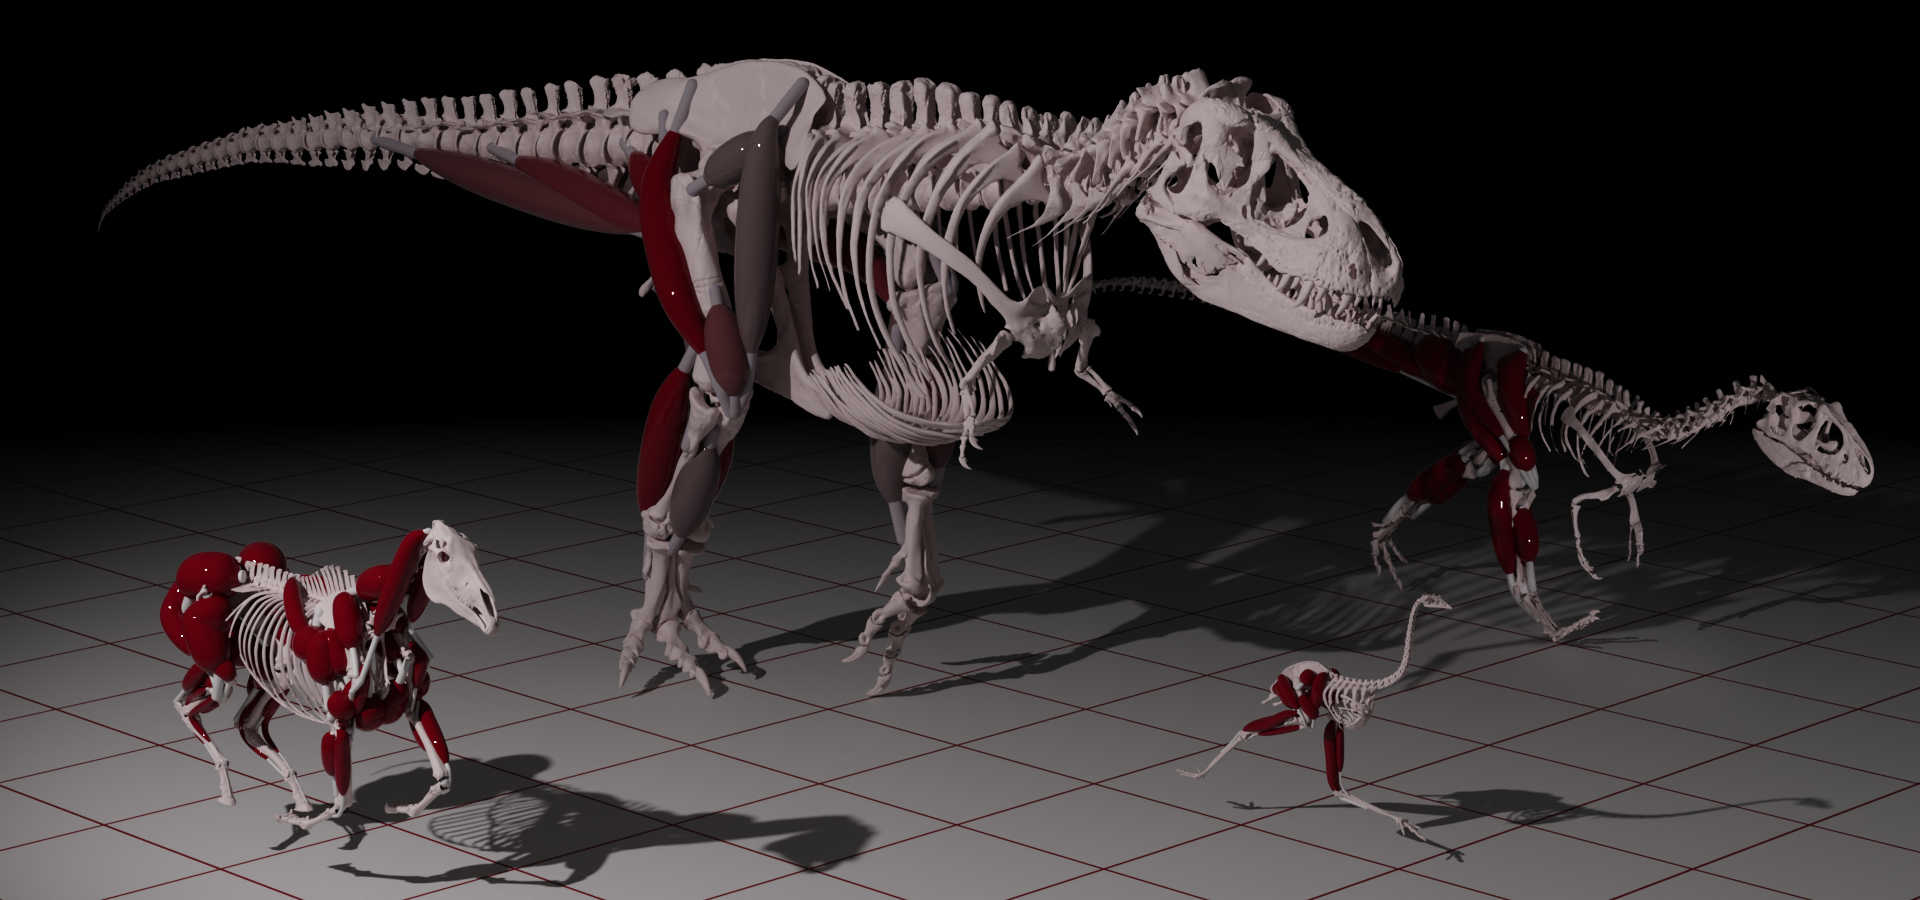
\includegraphics[width=\textwidth]{figures/cover_pic.png} % Add image
    \end{figure}
    \setcounter{figure}{0}
    \vspace{20pt} % Add vertical space between image and author section
    
    {\Large \textbf{Pasha van Bijlert}}\\
    \vspace{10pt}
    \textbf{pashavanbijlert@gmail.com}\\
    \textbf{Github Repository:} \href{https://github.com/PashavanBijlert/MuSkeMo}{Github} \\
    \textbf{Bug Reports and Feature Requests:} \href{https://github.com/PashavanBijlert/MuSkeMo/issues}{Submit an issue on Github} \\
    \vspace{20pt}
    {\large Version 0.9.75} \\
    {\large \today}
\end{center}

\vspace{20pt} % Add space before citation note
\noindent
\textbf{How to cite MuSkeMo:} I am preparing a publication to submit for peer-review describing MuSkeMo. Until that is available, please cite the preprint on bioRxiv if you used MuSkeMo for your work.

\noindent
PA van Bijlert. \textit{MuSkeMo: Open-source software to construct, analyze, and visualize human and animal musculoskeletal models and movements in Blender}. bioRxiv (preprint) 2024.12.10.627828; doi: \href{https://doi.org/10.1101/2024.12.10.627828}{10.1101/2024.12.10.627828}.

\vfill  % This pushes the content to the bottom of the page

\newpage  % Page break to separate the title page from the rest of the document


\tableofcontents

\newpage
\section{Introduction}

MuSkeMo is a tool for musculoskeletal modeling in \href{https://www.blender.org}{Blender}. MuSkeMo allows you to translate biological 3D scans to useful biomechanical information, in the form of full models or model components. These can then be used for further analysis within Blender, or exported for simulations in other biomechanical software. Simulation trajectories can be imported back into MuSkeMo to make publication-ready stills and videos, using Blender's built-in raytracing rendering. MuSkeMo can also be used for 3D landmarking and for simply calculating inertia tensors from 3D scans.

This MuSkeMo documentation file is meant to complement the \href{https://youtube.com/playlist?list=PLfgxaucAWlEp5-cavvXmdrTIWYT_tgZYK&si=Cdl9MchuLP5aRJNL}{video tutorial series on YouTube}. Users are encouraged to download the sample datasets and follow along with the video tutorials.
This documentation is focused on features specific to MuSkeMo, and where necessary provides suggestions regarding Blender settings and features. Because Blender can be overwhelming at first, new users are recommended to follow the "Donut tutorial" series by BlenderGuru on Youtube. For Blender-specific questions, the reader is referred to the extensive \href{https://docs.blender.org/}{Blender documentation}. MuSkeMo currently officially supports Blender 4.1 -4.5.

\subsection{Installation instructions}

To download: Go to the \href{https://github.com/PashavanBijlert/MuSkeMo/releases}{releases page} on the Github repository, and download the most recent version of "MuSkeMo.zip". The .zip file is used to install the plugin, but also contains a folder with utility functions (e.g., for OpenSim conversion).

To install (Fig. \ref{fig:installation}): In Blender v4.1, go to Edit → preferences → Add-ons and then click "Install...", and then select your downloaded zip file. Then type in "MuSkeMo" in the search bar of the addon window, and enable the plugin by pressing the check mark. If using Blender 4.2+, the install button is replaced with a downwards arrow, which gives ``Install from disk''.

\begin{figure}[h]
    \centering
    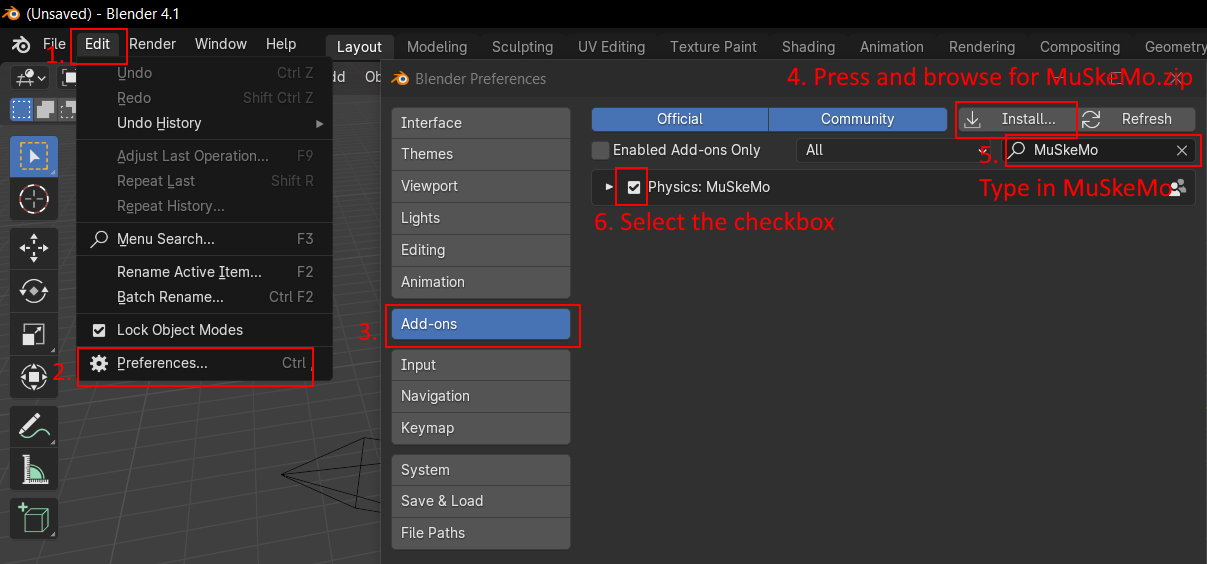
\includegraphics[width=\textwidth]{figures/install_instructions.png} % Add image
    \caption{Installing MuSkeMo in Blender version 4.1. In 4.2+, Step 4 is replaced with pressing a downwards arrow and selection ``Install from disk''}
    \label{fig:installation}
\end{figure}

\subsection{Sample Datasets}
\label{sec:sampledataset}
Some of the \href{https://youtube.com/playlist?list=PLfgxaucAWlEp5-cavvXmdrTIWYT_tgZYK&si=Cdl9MchuLP5aRJNL}{video tutorials} use sample datasets, in which case they are also made available from Github. Currently, there is only one \href{https://github.com/PashavanBijlert/MuSkeMo/releases/tag/v0.x-sampledataset1}{sample dataset}, which includes two OpenSim models created using MuSkeMo, and compatible simulation trajectories so the user can create a video.

\subsection{Units}

MuSkeMo uses the following units:

\begin{itemize}
    \item \textbf{Spatial distance/position:} metres (\si{\metre})
    \item \textbf{Mass:} kilogram (\si{\kilogram})
    \item \textbf{Moment of inertia:} kilogram metre squared (\si{kg\,m^2})
    \item \textbf{Force:} Newton (\si{N})
    \item \textbf{Angle:} Degrees (\si{\degree}, only for pennation angle). Internally MuSkeMo uses radians during computations.
\end{itemize}


\textbf{WARNING:} Blender's default units are in metres. Many of the calculations in MuSkeMo are derived from the spatial position of individual points (vertices) of the 3D meshes. If you change the base units of Blender, these calculations are also implicitly scaled, and the units will no longer be correct (e.g., if you change Blender's base units to centimetres, linear dimensions will be off by a factor of 100, but volumetrics and inertial properties will be off by a factor of 100\(^3\)). MuSkeMo currently only officially supports metres as the base unit, correct scaling of the outputs if using other units is up to the user.

\subsection{A Note on Precision}
\label{sec:precision}

MuSkeMo is built using the Blender Python API, which internally uses double precision numbers (64-bit floating point, \(\sim16\) significant digits). However, Blender itself stores numbers using single precision (32-bit floating point, \(\sim8\) significant digits), including all 3D point and mesh data. This means that precision beyond 8 significant digits cannot be expected when using MuSkeMo. Single precision floats nevertheless have a very large range of numbers that can be represented—the smallest number that can be accurately reported is in the order of \(1\times10^{-38}\), approximately 1 million times smaller than the mass of an electron in kilograms.

Because computing inertial properties from 3D vertex data involves successive multiplications of single precision numbers, mass and inertial properties have an expected accuracy of 5-6 digits (see \ref{sec:inpropvalidation}).

\subsection{Orientations}

Orientations are represented as XYZ body-fixed Euler angles (see Appendix \ref{sec:eulerangles}) and as unit quaternions (see Appendix \ref{sec:quaternions}). Internally, MuSkeMo avoids Euler angles where possible because they are prone to gimbal lock, but popular simulators often use Euler angles by default (e.g., OpenSim, SCONE).


\section{Using MuSkeMo}

MuSkeMo lives in \href{https://docs.blender.org/manual/en/latest/interface/window_system/tabs_panels.html}{Blender panels} (Fig. \ref{fig:MuSkeMoUI}A). Panels can be interactively resized and collapsed, which can be useful depending on your screen size. The panels contain buttons that perform operations on the data (implemented as \href{https://docs.blender.org/api/current/bpy.types.Operator.html}{Blender Operators}). When hovering over a button, a tooltip appears that briefly explains the workings of the button in question. 

Nearly all functions in MuSkeMo work by selecting the correct objects in the scene, and then pressing a button. If the selected objects are incompatible with the button in question, MuSkeMo will display an error message that explains what went wrong. To make the user aware of what MuSkeMo object (types) are currently selected, each has a live selection display for the relevant object types.


Although Blender does support using a trackpad, it is substantially more intuitive to navigate with a mouse, and a keyboard with a separate numberpad. There are also certain settings that make navigation easier (see Section \ref{sec:MSM_glob_settings}).


\textbf{WARNING:} Ensure that 3D meshes (visual geometry and tissue outlines) have all their transformations applied before you start constructing the model. To do this, select the object, press \texttt{Control + A}, and select ``All transforms". This accounts for the way that Blender stores local transformations. When you move, rotate, and/or scale 3D models in Blender, these transformations are initially stored only locally in the object's data (an extra storage layer in Blender). This means that the object's position has not changed in 3D space, you have defined an extra local transformation that can easily be undone. Some of the functions in MuSkeMo may behave unpredictably unless transformations have first been applied.



\begin{figure}[htbp]
    %\vspace{-155pt}
    \centering
    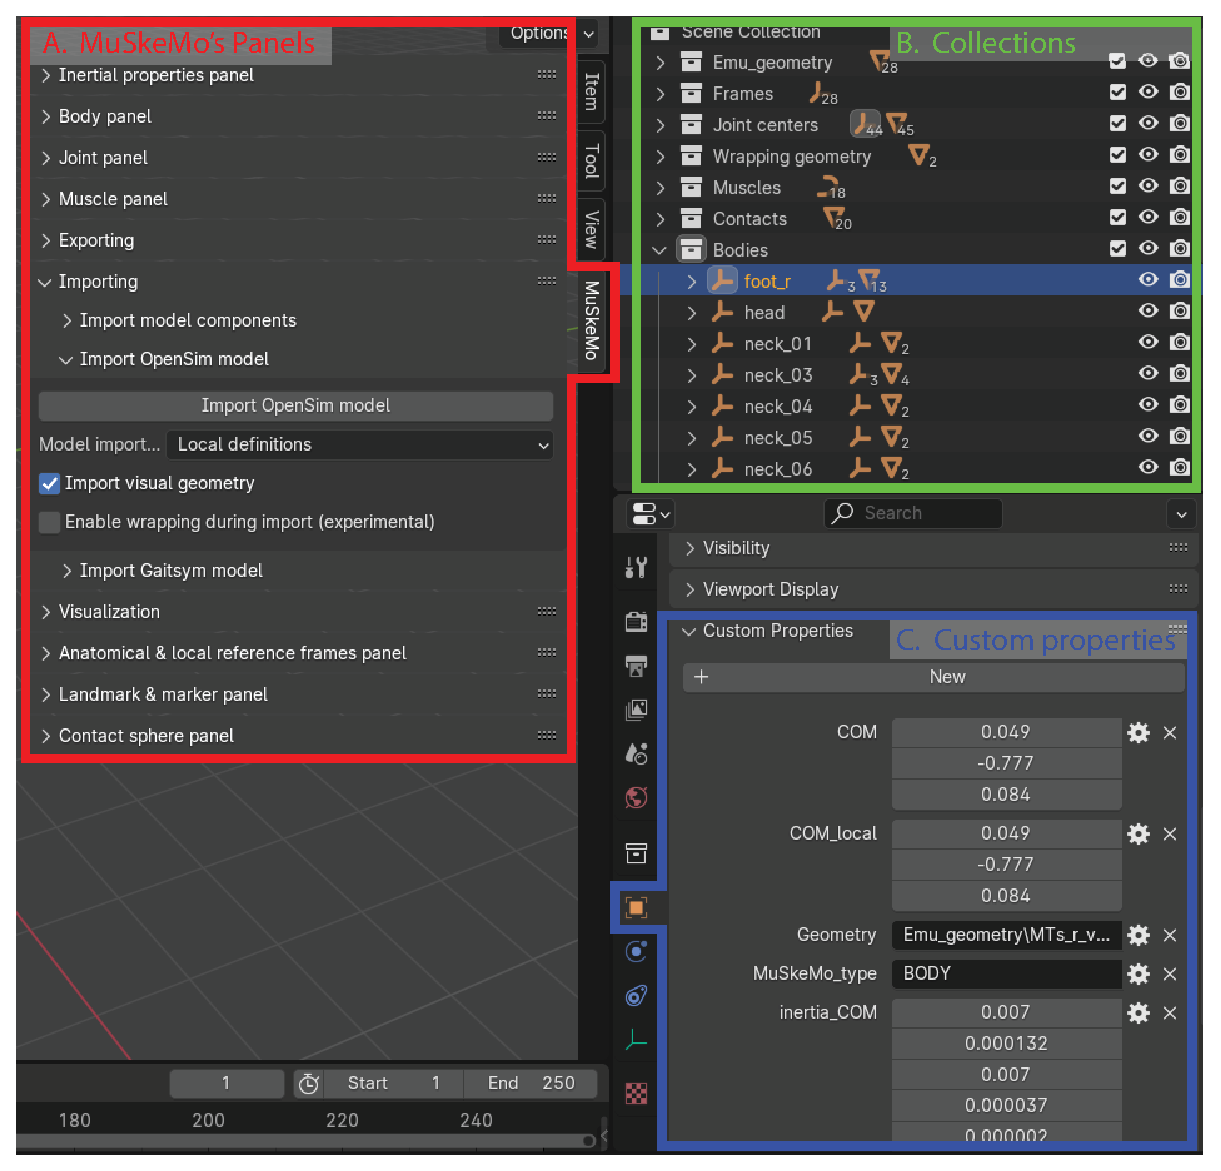
\includegraphics[width=0.99\textwidth]{figures/panels_coll_props.eps} % Add image
    \caption{A. All of MuskeMo's functionality can be accessed via these panels. The panels can be interactively resized and collapsed. B. After creating or importing model components, they are stored in Blender collections. If child objects are not visible, turn off object children in the outliner filter (see Section \ref{sec:MSM_glob_settings} C. A component's data are stored as custom properties. Press the yellow square, scroll all the way down, and open the Custom Properties dropdown}
    \label{fig:MuSkeMoUI}
\end{figure}

\subsection{Where MuSkeMo stores model data}
\label{sec:muskemodata}
All the model components and other user-created objects are stored in Blender \href{https://docs.blender.org/manual/en/latest/scene_layout/collections/collections.html}{Collections} (Fig. \ref{fig:MuSkeMoUI}B), which are essentially just folders. The collection names all have sensible defaults in MuSkeMo (e.g., "Bodies" for bodies), but can be changed if desired. The collection names are also used as the default filenames during import/export, but this is also customizable. By default, child objects aren't always visible in the collection that they're actually in (see Section \ref{sec:MSM_glob_settings}).

For each model component, data created by MuSkeMo are stored in Blender as \href{https://docs.blender.org/manual/en/latest/files/custom_properties.html}{Custom Properties} assigned to each object in question (Fig. \ref{fig:MuSkeMoUI}C, see also Section \ref{sec:DataTypes} on MuSkeMo Data Types).

\subsection{Model components and modifiers}

MuSkeMo creates a new \href{https://docs.blender.org/manual/en/latest/scene_layout/object/types.html}{Blender Object} for each model component. Blender has many different object types, but MuSkeMo mainly uses "Mesh", "Curve", and "Empty" (see \ref{sec:DataTypes} for a full specification of all the used data types). Objects in Blender do not interact with other objects, unless the user somehow defines their inter-relationships. MuSkeMo handles all of this under the hood. For instance, components such as contact spheres need to be parented to specific bodies in the model, and MuSkeMo handles this while also keeping track of these inter-relationships in "Custom properties" so they are exposed to the user (see \ref{sec:muskemodata}).

\label{sec:modifiers}
Combining parenting and Blender's native object types does not provide all of the required functionality. MuSkeMo extensively makes use of Blender's \href{https://docs.blender.org/manual/en/latest/modeling/modifiers/index.html}{Modifier system} for both generating and visualizing components. For instance, individual muscle curve points cannot be attached to bodies using Blender's parenting system, so MuSkeMo achieves this by adding a hook modifier for each curve point (see \ref{sec:muscle}). 

MuSkeMo uses both regular modifiers (which perform a predefined operation/modification on the object, e.g. the \href{https://docs.blender.org/manual/en/latest/modeling/modifiers/generate/bevel.html}{Bevel modifier} is used to round the edges of muscle visualizations), but also several custom-made Geometry nodes modifiers.

\href{https://docs.blender.org/manual/en/latest/modeling/geometry_nodes/index.html}{Geometry Nodes} modifiers are a very powerful way perform a customized sequence of operations on a specific object. MuSkeMo uses custom-made geometry nodes modifiers for muscle visualization (\ref{sec:simplemuscleviz} and \ref{sec:volmuscleviz}), muscle wrapping \ref{sec:musclewrapping}, creating parametric wrap geometry \ref{sec:wrapgeom}, amongst other features. The most important inputs for most MuSkeMo's custom Geometry nodes are accessible from the modifier panel itself, but advanced Blender users can also dive into the nodes themselves for more in depth modifications to their behavior. Where possible MuSkeMo tries to reuse node groups, which means that it is possible to make global changes to geometry node behavior by changing the parameters of a single node group. For example, the visualization of all the muscles can be changed by modifying the underlying node groups (\ref{sec:simplemuscleviz} and \ref{sec:volmuscleviz}).

By default, MuSkeMo color codes each component (see \ref{sec:defaultcolors} for details).


\subsection{Blender Auto Save}

Blender is quite stable, but it is possible for it to crash. Fortunately, by default, Blender has an Auto Save function. After a crash, restart Blender, and go to File, Recover, Auto Save. Remember to save the recovered file.

\subsection{Default pose}
\label{sec:defaultpose}
Constructing a model in Blender provides the user with a lot of freedom to interactively repose model elements during model construction. However, many of the computations are only valid in the specific pose they are computed in. For example, when computing mesh inertial properties using the inertial properties panel (\ref{sec:inproppanel}), the inertal properties in the global reference frame are only valid as long as the orientation and position (the pose) of the mesh do not change. Similarly, object positions and orientations with respect to parent frames (\ref{sec:frame}) are only valid during export if their relative positions and orientations remain unchanged. 

To prevent incorrect exports, MuSkeMo keeps track of the 'default\_pose', which is the pose in which the relevant computation was performed. If the user tries to perform an operation that can only be performed in the default pose, the operation is cancelled (with an error message). In that situation, you must reposition the model components back into the default pose before exporting. MuSkeMo provides a button for this: "Reset to default pose", available from the Global settings panel (sec. \ref{sec:MSM_glob_settings}), the Joint panel (sec. \ref{sec:jointpanel}), the Body panel (sec. \ref{sec:bodypanel}), the inertial properties panel (sec. \ref{sec:inproppanel}), and the export panel (sec. \ref{sec:exportpanel}). The button works by selecting one or multiple objects that have a default pose, and then pressing the button. If a single object is selected and it is part of a model, MuSkeMo traverses the model until it finds the root joint or body (i.e., the component at the top of the parent hierarchy), and then resets all the joints and bodies to their default pose. If multiple components of the same model are selected, MuSkeMo only performs the operation once (because they will both have the same root). If multiple disjointed objects are selected, MuSkeMo will reset the default pose for all the separate sections (including individual meshes with inertial properties).

Alternatively, if the user wishes to export the model in the changed pose, it is necessary to recompute all the model parameters in this new pose. For inertial properties and bodies, this means recomputing and reassigning the inertial properties, for other components it means detaching and reparenting the objects.

% \subsection{Example Model Building Workflow}

% Model building approaches can vary depending researcher preferences, research questions, and intended purpose of the model (8-15). This section provides a possible workflow to construct a model using MuSkeMo, for predictive simulations in third party simulators. However, MuSkeMo's many features make it suitable for a variety of other biomechanical and/or morphological analyses.

% \begin{enumerate}
% \item	Import a skeletal mesh into Blender, partition it into relevant body segments, and position it into a neutral posture (Fig 1A). Optionally, retrodeformation techniques can be applied if the meshes are deformed fossil specimens (16).
%  \item Import tissue outline meshes (acquired using CT scans), partition those into equivalent segments, then use MuSkeMo's ``Inertial properties panel" to estimate body mass properties of these meshes (Fig 1B). The user can specify a density, and which meshes to apply these densities to. After pressing the relevant button, the inertial properties are automatically computed. If tissue outline meshes are not available (e.g., when analyzing a fossil taxon), MuSkeMo's convex hulling features (Fig 1B) can generate them using empirical equations from the literature (17,18).
% \item	Create rigid bodies in MuSkeMo's ``Body panel".  Each rigid body should have a unique name. Rigid bodies can represent the combined inertial properties of one or more meshes, as computed in the previous step: select one body and one or more meshes, then press ``Assign precomputed inertial properties". Optionally, the user can assign visual geometry to the rigid bodies for visualization purposes (e.g., the skeleton or tissue outline meshes acquired in steps 1 and 2): select a rigid body, and the target visualization meshes, and press ``Attach visual (bone) geometry".
% \item	In MuSkeMo's ``Joint panel", create joints for each desired joint (link, articulation) in the model (Fig 1H). The position and orientations of the joints can be set manually (using Blender's transformation tools), or alternatively by fitting geometric primitives to portions of the skeleton (Fig. 1D). This option is available under ``Joint utilities", in the Joint panel. The ``match position" and ``match orientation" buttons automatically transform selected joints to target fitted geometry (or other target objects in the scene). Parenting is handled by the panel if the user selects one rigid body and one joint, and presses the ``Assign parent body" or ``Assign child body" buttons.
% \item	Create muscles in MuSkeMo's ``Muscle panel" (Fig. 1E) Muscle points are added to Blender's 3D cursor, provided the user selects a body to which the point will be parented. Before adding a muscle point, the user can reposition the 3D cursor with ``Shift + right mouse button". Once a muscle point is created, it can be repositioned by bringing the muscle point into Blender's ``Edit mode", which is accessible using the ``TAB" key. Optionally, the user can add wrapping to a muscle in this panel, or plot moment arms to iteratively reposition the muscle points. It is possible to assign contractile properties to each muscle via its Custom Properties (see Methods, and Supplementary File S1). MuSkeMo can display a muscle's length in real time, which enables the user to determine suitable optimal fiber lengths and tendon slack lengths by manually moving the model through different postures (see [9,12,19] for details).
% \item	Define contact sphere positions in the ``Contact sphere panel" (Fig. 1G). The approach is very similar to creating joints, except that contact spheres are placed on the 3D cursor location.
% \item	Optionally, the user can create frames in the ``Anatomical and local references frames panel" (Fig. 1C). These frames can either be positioned and oriented manually, or constructed with the help of landmarks (using cross-products, as described in [20]). When using landmarks, these first need to be created using the ``Landmark & marker panel". Landmark-based frames can be constructed with an arbitrary primary axis (X,Y, or Z) and arbitrary secondary plane (one of the two remaining unused directions), resulting in six possible ways to construct right-handed reference frames using landmarks (see the Supplementary File S1, the manual, for details).
% \item	It is possible to reflect all the created model elements in MuSkeMo's ``Reflection panel" to create a symmetric model (Fig. 1F). This requires following a consistent naming convention when creating sided model elements (all right-side model components names should end with ``\_r" and vice-versa, e.g., ``thigh\_r", ``knee\_r" , etc.).
% \item Export all model components using the ``Export panel". Model components are exported as .CSV files. Users can process these in their simulator of choice, see for example the OpenSim conversion Matlab script provided in the ``MuSkeMo Utilities" folder.
% \end{enumerate}

\section{MuSkeMo's Panels}
This section describes all of MuSkeMo's panels and how to use them. Most of MuSkeMo's features work by selecting the correct combination of objects, and then pressing one of the buttons in the panels. MuSkeMo's panels show you how many and what types of objects (e.g., "BODY") you have selected, and will give an explanatory error message if you try to use a panel incorrectly (e.g.,: assigning a parent body to a joint requires selecting one body and one joint, and MuSkeMo informs you if you didn't do this). Most of the panels also allow you to create new objects, which means you have to type in a (unique!) object name and press a button. 

\subsection{MuSkeMo Global Settings Panel}
\label{sec:MSM_glob_settings}
The Blender user interface has several default settings that do not work well with MuSkeMo. By default, Blender forces the Z-axis as the "up" direction in the viewport. The International Society of Biomechanics assumes Y as the up direction. To achieve this, the user should set the view rotation setting to "Trackball", and use "orbit around selection". The "MuSkeMo Global Settings" panel provides a button that does this automatically: "Set recommended navigation settings". 

The panel also has a button named "Set object children visibility". This toggles off "Object Children" in the outliner. In Blender's behavior, objects are placed under their parents in the outliner, but this would for instance result in a body being placed under the parent joint in the "Joint collection", instead of in the "Body collection". Turning off "Object children" avoids this behavior. MuSkeMo automatically calls the "Set object children visibility" operator when the user creates a Body, Joint, or Muscle for the first, so in most cases, you will not need to set this yourself. However, if you find yourself in a situation where you cannot find your objects in the outliner, even though you can clearly see them in the scene, this button may solve your problem.


\subsection{Mesh tools panel}
This panel combines several tools that are generally useful when manipulating or repositioning meshes. Some of these are also available in different panels (e.g., the intersection checker is also made available in the visual geometry subpanel \ref{sec:visgeomsubpanel}).

\subsubsection{Mesh alignment}
\label{sec:meshalignment}

Aligning 3D meshes in space is a common task when dealing with 3D biomechanical data. To use MuSkeMo's mesh alignment tool, simply select two meshes, designate which mesh is the target (stationary) object, and which one is the free mesh (which will be moved to achieve alignment), and then press ``Align Meshes''. The alignment assumes that you have approximately aligned the meshes yourself, and that they have the same scale.

The alignment uses an iterative closest point algorithm (point to plane, following \cite{chenObjectModelingRegistration1991}), using Blender's \href{https://docs.blender.org/api/current/mathutils.kdtree.html}{KD-tree} module to improve performance \cite{zhangIterativePointMatching1994}. Performance is further improved with (random) subsampling (see \cite{rusinkiewiczEfficientVariantsICP2001}), and the subsampling is slowly ramped down after several iterations so the final alignment is based on the entire meshes.

The following settings are available:


\begin{enumerate}
    \item \textbf{Free Object.} Selects which object is allowed to move during ICP point-to-plane mesh alignment.
    
    \item \textbf{Max Iterations.} Maximum number of iterations performed during ICP point-to-plane mesh alignment. Higher values may improve accuracy but increase computation time.
    
    \item \textbf{Tolerance.} Error tolerance used to determine convergence of the ICP alignment. Smaller values enforce stricter convergence at the cost of runtime. Values below $10^{-8}$ are unlikely to improve results significantly.
    
    \item \textbf{Start Sample Ratio.} Fraction of points used for sub-sampling at the beginning of the ICP process. A lower ratio speeds up early iterations while maintaining coarse alignment.
    
    \item \textbf{End Sample Ratio.} Should be higher than Start Sample Ratio. Fraction of points used for sub-sampling at the end of the ICP process. If you set this to lower than 1, the final iterations will still use a sample ratio of 1 (ensuring that the final alignment is based on all points).
    
    \item \textbf{No. iterations before end ratio.} Number of iterations before the sample ratio reaches the defined end value. Controls how quickly the sampling density increases during ICP.
\end{enumerate}


\subsubsection{Checking geometry intersections}
\label{sec:intersectionchecker}

MuSkeMo implements a mesh intersection checker, which is used by the pose sampling scripts in the MuSkeMo utilities folder (see sec. \ref{sec:posesampling}). This works via Blender's \href{https://docs.blender.org/api/current/mathutils.bvhtree.html}{BVHTree module}, which is an implementation of Bounding Volume Hierarchies \cite{ericsonBoundingVolumeHierarchies2005}. Essentially, the mesh is bounded by successively smaller objects in a nested tree structure, and Blender's BVHTree traverses down the tree while checking whether these bounding objects intersect with other objects in the scene. By starting with large bounding volumes, and only traversing the tree if the larger objects trigger an intersection, this is a computationally efficient way of checking for intersections. The \href{https://en.wikipedia.org/wiki/Bounding_volume_hierarchy}{Wikipedia page on Bounding Volume Hierarchies} also gives an accessible explanation on how this works.


\subsection{Inertial properties panel}
\label{sec:inproppanel}

The main goal of this panel is to compute inertial properties from 3D volumetric meshes, eg. from CT-segmentations or surface scans.
Inertial properties are not dynamic, if you move the 3D meshes or would like to change their densities, you must recompute their inertial properties, otherwise COM, mass, and or inertia can be outdated. MuSkeMo warns you if this has occured, by tracking the 'default\_pose' of each mesh as a custom property (see \ref{sec:defaultpose}). Density can only be changed by changing the 'Segment density' in the panel and recomputing the object's inertial properties.

To compute the volumetric inertia tensor (with elements in the unit \si{m^5}) of a triangular mesh, MuSkeMo implements the solution derived and presented in \cite{eberlyGamePhysics2004}. This gives an exact solution for the volumetric moments of inertia of a closed, triangulated mesh, based on the Divergence Theorem. This algorithm requires the mesh to be triangulated and watertight to provide meaningful results, and MuSkeMo alerts the user if this is not the case. The volumetric tensor is multiplied by density (in \si{kg m^{-3}}) to acquire the inertial tensor elements (in units \si{kg m^2}). 

It is possible to change the density property of an object, after which you will have to select the object and rerun "Compute for selected meshes". See \ref{sec:inpropvalidation} for a validation of the outputs.

\subsubsection{Generate minimal convex hulls}
Several studies have used convex hulls as the starting point for estimating inertial properties of (extinct) animals directly from full skeletons \cite{sellersMinimumConvexHull2012,brasseyScalingConvexHull2014,brasseyConvexhullMassEstimates2016,brasseyVolumetricTechniqueFossil2018,coathamConvexHullEstimation2021,macaulayDecouplingBodyShape2023,wrightVolumetricElementscalingMass2024,batesRunningPerformanceAustralopithecus2025}.
In this subpanel, you can automatically generate convex hulls around (skeletal) meshes in a collection, and then apply methods from the literature to reconstruct the inertial properties.

You have to designate the "Skeletal mesh collection" where your skeletal meshes are located. This defaults to the "Geometry" collection, but it can also be a different collection. Each separate object in the collection will receive its own convex hull, so the meshes in the collection should represent functional body segments. See \cite{sellersMinimumConvexHull2012,coathamConvexHullEstimation2021, macaulayDecouplingBodyShape2023} for examples. Convex hulls are placed in a new collection. 

The recommended workflow is to organize all the skeletal meshes in a single collection. Ensure that all the skeletal meshes contain the correct segment names in their full name (see below). Then, generate the minimal convex hulls, and use one of the expansion modes to expand those convex hulls.


\subsubsection{Expand convex hulls} 

Both the expansion panels (arithmetic and logarithmic) work with segment names and corresponding scale factors or logarithmic parameters. If only "whole\_body" is typed in as Segment name 1 (with no other segment names defined), all the objects in the target collection will be treated as one - in arithmetic mode, all objects are scaled by a single factor, in logarithmic mode, all object volumes are summed before determining the whole-body scale factor. 

If segment 1 is not "whole\_body", or if you have more than one segment name defined in the panel, MuSkeMo tries to match whatever segment names you have typed into the panel to the names of the objects in your target collection. E.g., if you've typed "neck" as one of the segment names in the panel, with a corresponding scale factor, all the objects in Convex hull collection that have the case-sensitive word "neck" in their name will be expanded by the scale factor (e.g., "neck\_1", "neck\_prox.obj", but not "Neck\_1" and also not "torso"). The "Expansion Template" dropdown menu gives several presets from the literature, and you can customize them if desired.

MuSkeMo assumes you want bilaterally symmetric models, and therefore when using the expansion functions, MuSkeMo generates bilaterally symmetric expanded hulls for the following segments: "head", "neck", "torso", "tail" (meaning the target skeletal objects should have those strings in their names). Furthermore, MuSkeMo also applies directional scaling. The following segments are scaled about the Y and Z axes (and thus not the X axis): "head", "neck", "torso", "tail", "forearm", "hand", "toe". All other segments are scaled about the X and Z axes. The resultant scaled shapes may not be very biologically realistic. You could add a "Maintain volume" constraint and change the shape in Blender (this was a suggestion by Matt Dempsey). Apply the constraint after you are satisfied.

Under \textbf{Expand convex hulls - arithmetic}, you can use arithmetic expansion factors (i.e., linear scale factors) to scale your hulls. If a segment initially has a volume of 1 \si{m^3} and a scale factor of 1.2, the resultant segment will have a volume of 1.2 \si{m^3}. 

\begin{itemize}
    \item \textbf{Custom:} Type in the segment names, and the desired scale factor.
    \item \textbf{Macaulay 2023 Bird:} The per-segment "Bird" average expansions from Macaulay et al. 2023 \cite{macaulayDecouplingBodyShape2023}, supplementary data S6.
    \item \textbf{Macaulay 2023 Non-Avian Sauropsid:} The per-segment "Croc\_Lizard" average expansions from Macaulay et al. 2023 \cite{macaulayDecouplingBodyShape2023}, supplementary data S6.
    \item \textbf{Macaulay 2023 Average (Bird and Non-Avian Sauropsid):} The per-segment "Av." average expansions from Macaulay et al. 2023 \cite{macaulayDecouplingBodyShape2023}, supplementary data S6.
    \item \textbf{Sellers 2012 Large Mammals:} This is a "whole\_body" scale factor of 1.206 as described in \cite{sellersMinimumConvexHull2012}. This is the first introduction of this method, and the user is warned that the the Sellers 2012 curve was not calibrated using direct measurements of body mass for the analyzed skeletons \cite{sellersMinimumConvexHull2012}.
\end{itemize}

Under \textbf{Expand convex hulls - logarithmic}, it is possible to use log-transformed regression equations from the literature to scale your hulls. 
The equations have the form:

\begin{equation}
y = 10^a \cdot x^{b} \cdot 10^{\frac{\ln(10)}{2} MSE }
\label{eq:powercurve}
\end{equation}


This is known as an allometric power curve, and is the result of an ordinary least-squares regression of log-transformed data (see \cite{alexanderPrinciplesAnimalLocomotion2006,brasseyScalingConvexHull2014}). a is the y-intercept of the regression, b is the slope of the regression, x is the input convex hull volume, and y is the scaled hull volume. \(MSE\) is the mean squared error of the regression, also called the variance of the residuals, or $\sigma^2$, with $\sigma$ being the standard deviation or standard error of the residuals. The term $10^{\frac{\ln(10)}{2} MSE }$ is used for a bias correction to account for the fact that we are transforming log-transformed data back to arithmetic units, see \cite{baskervilleUseLogarithmicRegression1972,sprugelCorrectingBiasLogTransformed1983,smithLogarithmicTransformationBias1993}. $MSE$ is assumed to be computed in base-10 logarithms, hence the extra factor $\ln(10)$ \cite{sprugelCorrectingBiasLogTransformed1983,smithLogarithmicTransformationBias1993}. Where $MSE$ was not or inconsistenly reported by the original studies, MuSkeMo sets it to 0 in the expansion templates, which implies a small, systematic, underestimation of the predictions by the power curve. By unticking the box "Apply Bias Correction", the bias correction is not applied during expansion even if the template has a value pre-filled (i.e., setting MSE to zero during the computations).


\begin{itemize}
    \item \textbf{Custom:} Type in the segment names, and the desired scale factor.
    \item \textbf{Macaulay 2023 Logarithmic Bird:} The logarithmic per-segment "Bird" average expansions from Macaulay et al. 2023 \cite{macaulayDecouplingBodyShape2023}, supplementary data S4.
    \item \textbf{Macaulay 2023 Non-Avian Sauropsid:} The logarithmic per-segment "Non avian sauropsid" average expansions from Macaulay et al. 2023 \cite{macaulayDecouplingBodyShape2023}, supplementary data S5.
    \item \textbf{Macaulay 2023 Average (Bird and Non-Avian Sauropsid):} The logarithmic per-segment "all taxa" average expansions from Macaulay et al. 2023 \cite{macaulayDecouplingBodyShape2023}, supplementary data S3.
    \item \textbf{Coatham 2021 Logarithmic Mammal (rewritten volumetric):} The logarithmic per-segment mammal equations from Coatham et al. 2021 \cite{coathamConvexHullEstimation2021}. This implementation factors out the density to transform them into volumetric expansions, see below. MuSkeMo squares their ``root mean squared errors'' (RMSE) to acquire mean squared errors ($MSE$) in eq. \ref{eq:powercurve}, but sets it to zero for the torso segment because the reported RMSE for the torso (3.42) leads to a bias correction factor of \(7 \cdot 10^{5}\).
\end{itemize}


Coatham et al. directly regressed convex hull mass against CT-based tissue outline mass, assuming a constant density of \(\rho\) = 1000 \si{kg m^{-3}}. Because this essentially gives a constant factor, these can be factored out to create volumetric equations as follows:

\begin{equation}
\begin{aligned}
y \cdot \rho &= 10^a \cdot (x \cdot \rho )^{b} \cdot 10^{\frac{\ln(10)}{2} MSE } \\
y &= 10^a \cdot \rho^{b} / \rho  \cdot x^{b} \cdot 10^{\frac{\ln(10)}{2} MSE } \\
y &= 10^a \cdot \rho^{b - 1} \cdot x^{b} \cdot 10^{\frac{\ln(10)}{2} MSE }
\end{aligned}
\end{equation}


Here, y is still the expanded volume, and x is the convex hull volume. The original a can then be replaced with: 


\begin{equation}
a_{\text{new}} = \log_{10} \left( 10^a \cdot \rho^{b - 1} \right)
\end{equation}




\subsubsection{Whole body mass from convex hulls}

Several studies have regressed total body mass to summed convex hulls of the entire body, as an approach to estimate total body mass from skeletons \cite{brasseyScalingConvexHull2014,brasseyConvexhullMassEstimates2016,brasseyVolumetricTechniqueFossil2018,wrightVolumetricElementscalingMass2024}. 

For the mass estimation equations, x is the summed volume of the convex hulls of all the body segments in \si{m^3}, and y is the computed total body mass in \si{kg}.

This subpanel sums all the convex hull volumes in a designated collection, then uses the user-selected empirical equation to compute total body mass (in kg). This assumes the convex hulls are of the complete skeleton (including both left and right sides). Available equations are:

\begin{itemize}
    \item \textbf{Wright 2024 Logarithmic Tetrapods:} Regression equation from \cite{wrightVolumetricElementscalingMass2024}, based on primary data, and reused data from \cite{coathamConvexHullEstimation2021} and \cite{sellersMinimumConvexHull2012} (the latter includes estimates instead of measurements of total body mass)
    \item \textbf{Brassey 2018 Logarithmic Primates:} from \cite{brasseyVolumetricTechniqueFossil2018}.
    \item \textbf{Brassey 2016 Logarithmic Pigeons, Eviscerated:} from \cite{brasseyConvexhullMassEstimates2016}, using the eviscerated pigeons equation.
    \item \textbf{Brassey 2016 Logarithmic Pigeons, Combined:} from \cite{brasseyConvexhullMassEstimates2016}, using the combined pigeons equation.
    \item \textbf{Brassey 2014 Logarithmic Primates:} from \cite{brasseyScalingConvexHull2014}.
    \item \textbf{Brassey 2014 Logarithmic Mammals:} from \cite{brasseyScalingConvexHull2014}, this reuses data from \cite{sellersMinimumConvexHull2012} which includes body mass estimates instead of direct measurements.
\end{itemize}

The original Brassey et al. 2016 \cite{brasseyConvexhullMassEstimates2016} pigeon equations assume volume is  \si{mm^3}, and provide the mass in \si{g}. To convert the output to kilograms (multiply by \(10^{-3}\)) and allow the input to be in \si{m^3} (multiply input by \(10^9\)), it is possible to rewrite equation \ref{eq:powercurve}.

\begin{equation}
y = 10^{-3} \cdot 10^a \cdot (x \cdot 10^9 )^{b} \cdot 10^{\frac{\ln(10)}{2} MSE }
\end{equation}

After rewriting, this gives:

\begin{equation}
    a_{new} = a - 3 + 9\cdot b
\end{equation}

Wright et al. \cite{wrightVolumetricElementscalingMass2024} multiply the summed convex hull volume by a density of \(\rho\) = 1000 \si{kg m^{-3}} before applying their power curve. This implies that mass scales with \(\rho^b\) in their predictive model.




\subsection{Body panel}
\label{sec:bodypanel}

Create new bodies by typing in a (unique) name, and then pressing the 'Create new body' button. The newly created body will have all 'NaN's as inertial properties, and will be centered at the origin. Once you assign rigid body parameters, the body will be moved to the correct position in the global reference frame. A body's position is always its center of mass in the global frame, and its orientation is always aligned with the global frame.

You can assign rigid body parameters in two ways. The recommend approach is to assign values that were computed for meshes in the inertial properties panel (see \ref{sec:inproppanel}). A single body can represent the combined inertial properties of more than one mesh. MuSkeMo computes the combined inertial properties using the parallel axes theorem \cite{valleryAdvancedDynamics2019,ruinaMechanicsToolsetStatics2019}. Simply select the target body, and 1+ source objects, and press 'Assign precomputed inertial properties'. MuSkeMo will give you an error message if you selected objects that don't have inertial properties precomputed, and the live selection boxes in the panel can help you with ensuring you have selected the correct (number of) objects. See \ref{sec:compositebodyvalidation} for a validation of these features.

It is also possible to assign inertial properties manually. This is not recommended, but it is possible by manually typing the values in the Body's custom properties. If going this route, the COM position can be updated using the button in the "Assign inertial properties manually" subpanel.


Inertial properties are not dynamic, if you move the source objects that the rigid bodies were based on, or change their densities, you must recompute all inertial properties of the body (see \ref{sec:defaultpose}). Otherwise COM, mass, and or inertia can be outdated. MuSkeMo warns you if you attempt to export inertial property data in a different pose than the default pose.

\subsubsection{Visual geometry (meshes)}
\label{sec:visgeomsubpanel}
In this panel, you can also attach visualization geometry (eg., bone meshes) to bodies. Select the meshes and the target body, and press the button.

The intersection checker (sec. \ref{sec:intersectionchecker}) is also available here, for easy access when articulating bone meshes.


\subsection{Joint panel}
\label{sec:jointpanel}

Create new joints by typing in a unique name and pressing 'Create new joint'. To and assign a parent or child body, select the joint and the target body, and press the respective button. 


Until joints are parented, there is no 'default pose' state being tracked (see \ref{sec:defaultpose}), and the global positions and orientations are listed as NaN in the custom properties (but are exported correctly if the user wants to export unparented joints). If a parent or child body has an anatomical (local) reference frame assigned, MuSkeMo automatically computes the relative positions and orientations in these frames as well. Orientations are stored as body-fixed, XYZ-Euler angles and as quaternions. All data that are created are included during export (if local frames are not assigned, these values will be NaN).

If you want to change a joint's position or orientation, detach the parent and child bodies first, or use the 'Match orientation' and 'Match position' buttons in the Joint utilities subpanel.

\subsubsection*{Joint coordinate names}

It is possible to define coordinate names in the joint panel. After exporting from MuSkeMo, the model conversion scripts (e.g., MuSkeMo\_to\_OpenSim) will only add DOFs to model if they are named (e.g. hip\_angle\_r). If no coordinates are named for a joint, the joint is turned into an immobilized joint (e.g., WeldJoint in OpenSim). 

\subsubsection{Fitting primitive objects for joints}
\label{sec:primitivefitting}
In this panel, there are buttons that fit geometric primitives to a selected mesh (sphere, cylinder, ellipsoid, plane). Simply select a target mesh, and press one of the fitting buttons. The options are:

\begin{itemize}
    \item \textbf{Sphere (geometric).} Implements \cite{yesudasanFastGeometricFit2015}.
    \item \textbf{Sphere (least squares).} Implements \cite{Jekel2016}.
    \item \textbf{Cylinder.} Python implementation of the pseudocode in \cite{eberlyLeastSquaresFitting}. After implementing the fitting algorithm, MuSkeMo also uses the original vertex data to compute the height of the cylinder, based on the maximum z-span of the target vertices in the cylinder frame. The z-axis Euler angle is set to 0, because cylinders are rotationally symmetric about the long axis.
    \item \textbf{Ellipsoid.} This is a Python implementation provided courtesy of Mark Semple \cite{semplePyEllipsoid_Fit}, who converted Yuri Petrov's Matlab implementation. I modified it further to ensure right-handed coordinate systems.
    \item \textbf{Plane.} Simple implementation based on taking the covariance matrix of all the recentered vertex positions, which is conceptually identical to a principal component analysis. The best fitting plane must pass through the centroid of the data points \cite{pearsonLIIILinesPlanes1901}, which is used to recenter the data. The eigenvectors of the covariance matrix then encode the directions (principal components) of variance in the data \cite{jolliffeMathematicalStatisticalProperties2002}. The plane of best fit, in a least-squares sense, is orthogonal to the eigenvector corresponding to the lowest eigenvalue of the covariance matrix \cite{jolliffeMathematicalStatisticalProperties2002,pearsonLIIILinesPlanes1901}. This is taken as the Z-axis of the plane. The plane itself is taken as the basis spanned by the eigenvectors of the two largest eigenvalues. Right-handed coordinate systems are also ensured, by flipping the direction of one of the eigenvectors if necessary.
\end{itemize}

The functions will fit the entire mesh that you select, so if you want to fit a portion of the mesh (e.g., the femoral head), go through the following steps:


\begin{enumerate}
\item Select the target mesh
\item Press Tab to go into 'edit mode' in Blender
\item Select the portion of the mesh you would like to fit (easiest is to use face selection mode, and use the selection circle)
\item press shift \+ D to duplicate the selection
\item press P (for seParate), and then select "by selection".
\item press Tab to go out of edit mode.
\end{enumerate}

You have now copied a subsection of the mesh as a new mesh, which you can use as an input for one of the fitting functions. The duplicated section of the mesh is in the same collection as the original, and if the original mesh was attached to a BODY, so will this copied section. To prevent it being exported, move it to a different collection, and detach the mesh from the body using the button in the panel.

\paragraph {Matching joints to fitted geometry.} 

It is possible to match the position and/or oreintation of a joint to the fitted geometry, respectively. Simply select the target joint and a source geometry, and press the respective button. Child objects and parent objects are not transformed with the joint. Instead, only the joint's position or orientation is changed, and related data (e.g., pos\_in\_child) are recomputed automatically. 

\paragraph {Cycling through joint axes.} 
It is possible that the named axes of the fitted object do not correspond with how you would like the joint to behave (e.g., a aylinder's long axis is always the z-axis, but you may want that axis to align with the joint's x-axis). In this case, after using the match orientations button, use the "Cycle through joint axes" button. This button post-multiplies the joint's rotation matrix with the following permutation matrix (see also sec. \ref{sec:eulerangles}):

\begin{equation}
\mathcal{P} =
\begin{bmatrix}
0 & 0 & 1 \\
1 & 0 & 0 \\
0 & 1 & 0
\end{bmatrix}
\end{equation}


Cycling through it three times restores the original orientation.

\subsection{Muscle panel}

In this panel, you can define path-point muscles, view their lengths in realtime, analyze moment arms, and assign wrapping. Muscle points are added to the 3D cursor location, and parented to the selected Body (so you have to define bodies before creating muscles). New muscle points are always attached to the selected body, and muscles are placed in the user-designated "Muscles" collection. New muscles points are always added to the 3D cursor location. Press shift + right mouse button to reposition the 3D cursor. 

\subsubsection{Creating a muscle and adding points}

To create a new muscle, type a unique (unused) name in the text box, select a body, place the 3D cursor at the desired location, and press "Create new muscle". For each subsequent muscle points, select both the muscle and the target body, reposition the 3D cursor, and press "Add muscle point".

\textbf{Important:} MuSkeMo creates muscles using Blender's curves, and automatically hooks each point to the target body (see \ref{sec:muscle}). It is impossible to reposition the whole muscle, it can only be repositioned one muscle point at a time. To do this, select the muscle, and press "TAB" on your keyboard to go into \href{https://docs.blender.org/manual/en/latest/editors/3dview/modes.html}{EDIT mode}. In edit mode, you can select individual points and move them around by hitting G. Once you are satisfied, you can press TAB again to go out of edit mode.

It is possible to insert muscle points (instead of adding them at the end). To insert a point, select the point index after which you would like to insert a point (starting at 1), and press "Insert muscle point".

These instructions are also summarized in a "Muscle tooltips" box which can be hidden from view by deselecting the tick box.


\subsubsection{Visualization radius}
By default, muscles are visualized using a Geometry node modifier named "musc\_name\_SimpleMuscleViz" (see section \ref{sec:simplemuscleviz}). If this visualization option is used, you can change the visualization radius of all muscles simultaneously by using the "Update visualization radius" button after selecting a desired radius. Alternatively, you can manually tune individual radii of muscles by changing the input in the "SimpleMuscleViz" modifier.

If the volumetric visualization option is used for the muscles, visualization parameters can be tuned in the "VolumetricMuscleViz" modifier (see section \ref{sec:volmuscleviz} for details).

\subsubsection{View length in realtime}

This button adds a geometry node modifier named "LiveLengthViewer" to the active muscle. This allows the user to interactively pose the model and see how the muscle lengths change. This can be useful during muscle construction, and for tuning musculotendon parameters. The user can change the placement and the size of the text from the modifier inputs. %Add figure!
The node uses a custom node group named "LiveLengthViewerNodeGroup", which is shared between all muscles that have a length viewer modifier added to it. To disable the length viewer, remove the modifier from the muscle's modifier stack.


\subsubsection{Assigning wrapping}

You can use the ``Wrapping" subpanel to perform all the necessary steps to create and assign wrapping to a muscle. This includes creating wrapping object geometry (currently, only cylinders are supported), assigning parent bodies, and assigning muscles to wrap around an object. The panel also performs the reverse operations. Note that wrapping is currently only physically accurate (i.e., a true tangent solution) if each wrapped section is separated by at least one muscle point on both sides.

Wrapping geometries are also generated using geometry nodes (see \ref{sec:wrapgeom} for details), so that they can be interactively resized using the inputs in the wrapping object's modifier (see \ref{sec:modifiers}). When a WRAP is assigned to a muscle, it receives a very complex geometry nodes modifier (see \ref{sec:musclewrapping} for details). Changing the wrapping geometry dimensions (e.g., the cylinder's radius) also affects the dimensions of the muscle wrapping. Information on the dimensions of the wrapping object is carried over to the Muscle by creating a \href{https://docs.blender.org/manual/en/latest/modeling/geometry_nodes/geometry/read/named_attribute.html}{Named Attribute} in the Geometry node for the Wrapping object, which is then sampled in the Geometry node in the muscle wrapping node (see sec. \ref{sec:musclewrapping}).



\subsubsection{Moment arms}

MuSkeMo can compute a muscle's moment arms, about a single degree of freedom. Specify the muscle name in the top of the Muscle panel, and the "Active joint 1"  name in the Moment arms panel. You can choose between rotating about local x, y, or z axes, and the range (in degrees) over which the moment arms should be computed. MuSkeMo assumes that 0 degrees rotation is the current model's position. Angle step size determines how fine or coarse the joint range will be sampled. 

When a computation is succesful, a Python dictionary named "length\_data" is added to the muscles's custom properties. MuSkeMo computes the length of the target muscle over the desired joint range. Moment arms are computed using the principle of virtual work \cite{storaceFunctionalAnalysisRole1979,anDeterminationMuscleOrientations1984}, where \(r = -dL / d\phi \) (see section \ref{sec:momentarmvalidation} in the appendix for more details and a validation of MuSkeMo's moment arms). Only lengths are stored, moment arms are computed during plotting or export. If "Generate plot" is selected, moment arms are plotted straight away (see also \ref{sec:plotting}), which may be useful when constructing muscle paths. It is also possible to plot muscle lengths instead.

If "Export length and moment arm" is selected, a CSV (or other file, see \ref{sec:exportpanel}) is exported during moment arm computation. This requires setting a target export directory.

\textbf{Warning:} While the moment arms computed by MuSkeMo are physically accurate (Fig. \ref{fig:momentarmscombined}), they are slightly noisy when using wrapping, in the order of 0.015\% of the value of the moment arm, see \ref{sec:momentarmvalidation} for details. Readers intending to perform simulations using the exported moment arms themselves (instead of exporting full models for simulations), may want to smooth the wrapping moment arms before use.

\begin{figure}[htb]
    %\vspace{-155pt}
    \centering
    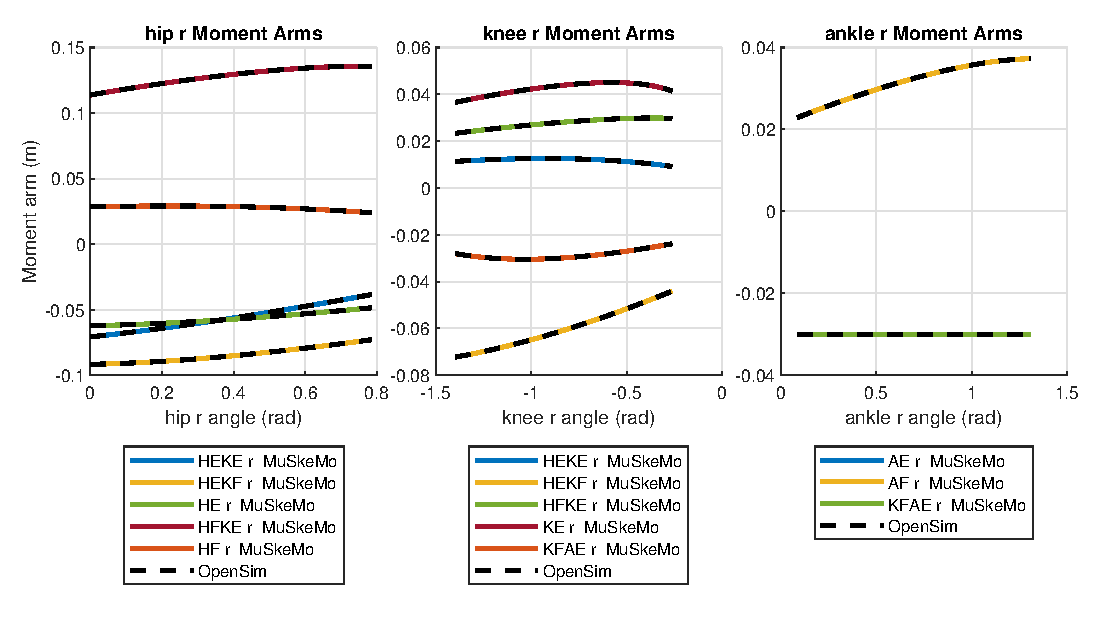
\includegraphics[width=1\textwidth]{figures/HKA_momentarms_emu.eps} % Add image
    \caption{Moment arms of the emu model from \cite{vanbijlertMusclecontrolledPhysicsSimulations2024}, computed by MuSkeMo and exported as .csv files, compared to those computed by OpenSim 4.0 using the Matlab API. See section \ref{sec:momentarmvalidation} for details. A python script that performs a moment arm analysis is provided in the Utilities folder \ref{sec:muskemoutilities}}. Note that this comparison gives identical results because the emu model uses only cylinder wrapping, and that each wrapping cylinder is separated by at least one muscle curve.
    \label{fig:momentarmscombined}
\end{figure}


\subsubsection{Plotting}
\label{sec:plotting}

The plotting subpanel provides the user with some flexibility to alter the plots. Change the parameters in the panel, and then press "(Re)generate a muscle plot", which updates the length or moment arm plot of the muscle in question. The plotter can only (re)generate a plot for muscles where "length\_data" were previously computed in the moment arms subpanel.

\FloatBarrier %forces the figure to display before starting the next section

\subsection{Anatomical \& local reference frames panel}
\label{sec:framepanel}

Construct anatomical and local reference frames (sec. \ref{sec:frame}) by assigning reference points to construct the axes directions, or via manual placement. The user defines a primary axis using two markers, and a temporary axis direction using a third, which together span a plane. The secondary axis is computed as perpendicular to the plane. The tertiary axis is mutually perpendicular to the first two axes, and lies on the same plane as the temporary axis. The reference frame is placed at the user-specified origin position.
You have to assign four positions:

\begin{itemize}
\item Primary axis start
\item Primary axis end
\item Temp axis (to define the plane together with the primary axis)
\item Frame origin (this can be the same marker as any of the previous three, if desired)
\end{itemize}

Each of these four positions is assigned by selecting a reference object, and pressing the corresponding ``assign" button. The position of those objects will be sampled when constructing the actual frame (using the "Construct Frames from landmark positions" button). It is recommended (but not mandatory) to use Landmarks as reference objects (see sec. \ref{sec:landmarkpanel} and \ref{sec:landmark}).

All three axes ( \(X\), \(Y\) and \(Z\)) can be selected as the primary axis, or the temporary axis to define the plane. It is also possible to place the new frame manually (in which case the frame is placed at the 3D cursor position). The panel thus has seven "Construction modes" which can be selected from a dropdown menu:

\begin{itemize}
    \item "Specify X-axis and Y-temp direction (for XY plane)".  
    \item "Specify X-axis and Z-temp direction (for XZ plane)".
    \item "Specify Y-axis and Z-temp direction (for YZ plane)".
    \item "Specify Y-axis and X-temp direction (for XY plane)".
    \item "Specify Z-axis and X-temp direction (for XZ plane)".
    \item "Specify Z-axis and Y-temp direction (for YZ plane)".
    \item "Manual placement (at 3D cursor position)"
\end{itemize}


As an example, when selecting the mode "Specify X-axis and Y-temp direction (for XY plane)": The frame will have its \(X\)-axis aligned to the direction specified by the primary axis start and end markers. The temp axis marker is used to define the \(XY\)-plane, and the \(Z\)-axis will be perpendicular to that plane (using a cross-product). The \(Y\) axis is found using another cross-product between the \(Z\) and \(X\) axes. This approach is commonly used to construct anatomical reference frames \cite{wuISBRecommendationsStandardization1995,wuISBRecommendationDefinitions2002,wuISBRecommendationDefinitions2005}.

Local reference frames have a position and an orientation with respect to the global reference frame. If the global frame is denoted with the letter \(\mathcal{G}\), then the position of an arbitrary frame in the global reference frame can be written as the following vector: \(\vec{v}_{\mathcal{G}}\). Internally, orientations are stored through rotation matrices. The rotation matrix that rotates a vector from the local \(\mathcal{B}\)-frame to the global \(\mathcal{G}\)-frame can be written as: \({}^{\mathcal{G}} \mathbf{R}_{\mathcal{B}}\). The vectors describing the axes directions in the global frame form three mutually orthogonal basis vectors, and they form the three columns of the orientation (rotation) matrix.

Orientations are exported as rotation (unit) quaternions (w, x, y, z), and also as body-fixed (intrinsic, active) XYZ-Euler angles (phi\_x, phi\_y, phi\_z, in rad) (see Appendices \ref{sec:eulerangles} \& \ref{sec:quaternions}). Euler angles are prone to gimbal lock. 

Anatomical / local frames can be assigned to a body by selecting one body and one frame, and pressing "Assign parent body". During parent body assignment, MuSkeMo computes inertial properties, joint positions and orientations, contact positions, and muscle path points with respect to these frames. This requires the transpose of matrix \({}^{\mathcal{G}} \mathbf{R}_{\mathcal{B}}\), namely: \({}^{\mathcal{B}} \mathbf{R}_{\mathcal{G}}\). This rotates a vector from the global \(\mathcal{G}\)-frame to the local \(\mathcal{B}\)-frame.

For an arbitrary point \(p\) expressed in \(\mathcal{G}\), MuSkeMo computes the transformation to \(\mathcal{B}\) as follows: 

\begin{equation}
\vec{p}_{\mathcal{B}} = {}^{\mathcal{B}} \mathbf{R}_{\mathcal{G}} \; (\vec{p}_{\mathcal{G}} - \vec{v}_{\mathcal{G}})
\end{equation}

For an arbitrary matrix \(\mathbf{I}\) expressed in \(\mathcal{G}\) (e.g., an inertial tensor with respect to the body COM), MuSkeMo computes the transformation to \(\mathcal{B}\) as follows \cite{valleryAdvancedDynamics2019}:

\begin{equation}
\mathbf{I}_{\mathcal{B}} = {}^{\mathcal{B}} \mathbf{R}_{\mathcal{G}} \;\mathbf{I}_{\mathcal{G}} \; {}^{\mathcal{G}} \mathbf{R}_{\mathcal{B}}
\label{eq:similaritytransformation}
\end{equation}

Readers familiar with linear algebra will recognize this as a similarity transformation, using a change of basis matrix \cite{layLinearAlgebraIts2016}.

\subsection{Landmark \& marker panel}
\label{sec:landmarkpanel}

Similar to muscle points, landmarks (sec. \ref{sec:landmark}) are added to the 3D cursor location. Type in a unique name for the landmark, place the 3D cursor in the desired location (shift + right mouse button), select the target mesh, and press the "create landmark" button. If the target mesh already has a parent body, you can also select the parent body instead. 

Landmarks are always parented to bodies (sec. \ref{sec:body}), not to the meshes themselves. Thus, if your target mesh does not have a parent body, MuSkeMo automatically creates one, and attaches the target mesh to that body as visual geometry (sec. \ref{sec:geometry}). MuSkeMo warns the user when this has occured. The newly created body will have the name ``[meshname]\_pbody''. When the user attempts to add a landmark to a mesh, MuSkeMo informs the user that the landmark was instead attached to the parent body.

If you are adding landmarks to visual geometry so that you can define local frames in the Anatomical \& local reference frames panel (sec. \ref{sec:framepanel}), it is recommended that you first create bodies with your desired names, and attach those visual geometry to those bodies. Otherwise, MuSkeMo will automatically parent the meshes to newly created bodies, and you will have to detach them later on.

Some people make a distinction between a landmark (projected onto a bone surface) and a marker (any reference position), hence the name of the panel.


\subsection{Contact panel}

Similar to muscle points, contacts are added to the 3D cursor location. Type in a unique name for the landmark, place the 3D cursor in the desired location (shift + right mouse button), and press the "create contact" button. Contacts can also be assigned a parent body, similar to joints.

\subsection{Export panel}
\label{sec:exportpanel}
You can export all the user-created datatypes via this panel. The individual exporters export all the data types from the user-designated collections (folders) in Blender. It is possible to export all the visual geometry to a subfolder.

MuSkeMo exports all the data with respect to both the global reference frame (origin), and body-fixed local reference frames. Orientations are exported as XYZ-Euler angle decompositions, and as quaternion decompositions.

Under export options, it is possible to configure other text-based filetypes for export (e.g., txt, bat), configure custom delimiters, and choose the number formatting in the exported files.


\subsection{Import panel}

You can currently import bodies, joints, muscles, frames, and contacts, if they are MuSkeMo-created CSV files.

\subsubsection{OpenSim model import}
\label{sec:opensimimporter}
MuSkeMo provides an OpenSim importer. This can import most of the components of an OpenSim model. The default behavior is to import models using local definitions, which means that all the local frames are created expicitly during model import. Each body's local \ref{sec:frame} a distinct object in the scene. If you are unsure which import mode to use, this is the option to select (which is why it is the default).

It is also possible to import models using global definitions - this is only useful for \textit{models created using MuSkeMo's conversion scripts, using the ``Global definitions" option}. In essence, this import mode assumes that all the component positions are defined as their position in the global frame, and for joints specifically, transformations in parent and child are both set to the global position and orientation. Local frames are not created. Because this mode assumes a very particular OpenSim model setup, there is less robust support for error-checking of the Geometry folder, and ``non-standard'' transform axes are not supported (see below).

During import, cylinder wrapping is supported (see \ref{sec:musclewrapping} and \ref{sec:wrapgeom}). MuSkeMo's wrapping definitions are different from OpenSim, and the importer tries to convert wrapping definitions. If the wrapping does not visualize correctly, it may be necessary to change the projection angle (combined with enabling "force wrap"), selecting "flip wrap", or "shortest wrap", depending on the situation. See \ref{sec:musclewrapping} for a full description of MuSkeMo's wrapping.

\textbf{Warning:} Blender does not allow \textit{any} object name to be reused. This means that all of your model components need to have unique names in MuSkeMo (so e.g., if a body is named 'shank\_r', and it has only one wrapping object, it still cannot be named 'shank\_r'. It would need a unique name such as 'shank\_wrap\_r'). If any component has a non-unique name, the OpenSim importer may fail. The importer currently checks whether frames and wrapping objects have non-unique names, but not other model components.

MuSkeMo does not support conditional or moving path points. These are automatically converted to regular path points during model import. For moving path points, the point position is selected that corresponds to the position when the controlling joint coordinate is equal to 0.

OpenSim joints have a "socket\_parent\_frame" and "socket\_child\_frame", which normally designates the names of the parent and child frames, respectively. The frames themselves are defined under the "frames" tag (usually PhysicalOffsetFrames), which also have names. It is possible that the "socket\_parent\_frame" or "socket\_child\_frame" does not correspond with either of the PhysicalOffsetFrames defined within the same joint. In this case, MuSkeMo assumes the user intends to use the actual PhysicalOffsetFrames as defined in the frames tag, and ignores the sockets. This is most likely a model error (inconsistent frame definitions), and MuSkeMo warns the user if this occurs during import.

OpenSim models with \href{https://simtk.org/api_docs/opensim/api_docs/classOpenSim_1_1CustomJoint.html}{CustomJoints} (and perhaps other joint types with a \href{https://simtk.org/api_docs/opensim/api_docs/classOpenSim_1_1SpatialTransform.html}{SpatialTransform}) can have \href{https://simtk.org/api_docs/opensim/api_docs/classOpenSim_1_1TransformAxis.html}{Transform Axes} that are different from the joint's principal axes, or have a specific user-defined order. In essence, Custom Joints allow users to define custom rotation application order about arbitrary axes, and allows translations about arbitrary axes as well (and the translation and orientation axes do not need to match). Such flexibility is not currently possible in MuSkeMo, R1 is always coordinate\_Rx (about the joint's local (1,0,0) axis), R2 is always coordinate\_Ry, and R3 is always coordinate\_Rz, and Tx, Ty, and Tz are about the same axes as the rotational axes. If a CustomJoint defines a different rotation order than Rx - Ry - Rz, and/or defines any of the transformations about different axes than (1,0,0), (0,1,0), or (0,0,1) (in that specific order), then the transform axes are treated as ``non standard". In this situation, MuSkeMo stores the name of the ``rotation1" coordinate as the ``coordinate\_Rx" (regardless of whether it originally encoded an x-axis rotation), ``rotation2" as ``coordinate\_Ry", and ``rotation3" as ``coordinate\_Rz", and the same for the translatory coordinates. The custom transform axes are stored as a Python dictionary in a custom property named ``transform\_axes". These transform axes are mapped onto the joint rotations themselves when importing trajectories (see \ref{sec:trajectoryimport}), using axis-angle rotations (see sec. \ref{sec:axisanglerotation}) in x-y-z order (thus preserving the user-defined custom order that was encoded in the CustomJoint). MuSkeMo warns the user during model import if such transform axes were detected and stored in a joint's custom data.
Non-standard axes are also assumed when the root joint's default pose is not aligned with the global reference frame.


OpenSim models require a joint that connects the model to the ground that decides the global degrees of freedom (MuSkeMo calls this a root joint). If a user creates an OpenSim model without defining a root joint, OpenSim automatically creates one (or multiple) \href{https://simtk.org/api_docs/opensim/api_docs/classOpenSim_1_1FreeJoint.html}{FreeJoints}, without any frames defined within the joint. If such a model is imported into MuSkeMo using local definitions, MuSkeMo creates these implicit frames at the origin, and guesses the intended OpenSim naming convention.


OpenSim allows the characters ``::" in the XML tags of their .osim format, which is not allowed in standard XML files. This is true for ``HuntCrossleyForce'' components, for instance. MuSkeMo automatically renames these tags during model import, although currently MuSkeMo does not import contact force parameters, so this is purely to prevent an XML import error.

\subsubsection{Gaitsym 2019 model import}

MuSkeMo includes a Gaitsym (2019) importer. It currently imports bodies, joints, muscles (DampedSpring elements are treated as muscles), contacts, and markers (as frames). Muscles that include wrapping are currently not supported, but limited wrapping support is planned in a future update. Visual geometry can be imported, but requires the user to type the name of the containing folder in "Gaitsym geometry folder". The geometries must be in a subdirectory of the model directory, and the name of this subdirectory must currently be manually typed into the panel.

It is possible to automatically apply a rotation to the entire model during import. This can be convenient because Gaitsym is generally geared towards the Z-axis being the "up" axis, whereas ISB recommends Y-up. To rotate a model from Z-up to Y-up, apply a -90 \degree rotation about the x-axis. Points simply get rotated, MOI gets transformed according to eq. \ref{eq:similaritytransformation} (although technically the transformation is now from one global frame to another). The same change-of-basis transformation is also applied to orientions (of joints, frames, etc.). The result is that the old Z-axis becomes the new Y-axis, and the old Y-axis becomes the new Z-axis.

\subsubsection{MuJoCo model import}
\label{sec:mujocoimporter}
MuSkeMo provides a MuJoCo importer. It should import most of the components of a MuJoCo model. It has only been tested on MuJoCo models converted from OpenSim using MyoConverter, made available \href{https://github.com/MyoHub/myoconverter/tree/main}{here}.

MuJoCo has a substantially different model format from most biomechanical simulators (see the \href{https://mujoco.readthedocs.io/en/stable/XMLreference.html}{documentation} of their model format). Although for the most part it is possible to convert MuJoCo models to MuSkeMo, the conversion will not result in a perfect correspondence in all cases. This is because of the way joints are defined in the \href{https://mujoco.readthedocs.io/en/stable/modeling.html#ctree}{MuJoCo kinematic tree}. In MuSkeMo, two BODIES (sec. \ref{sec:body}) have to be connected by a joint, even if the joint has no Coordinates (degrees of freedom). In contrast, bodies in MuJoCo can be directly parented to each other (which welds them together, in essence creating a composite body). When \href{https://mujoco.readthedocs.io/en/stable/XMLreference.html#body-joint}{joints} are added to a model, they are listed as subelements of the body they act on in the xml, (even though they technically act as a parent joint to that body). MuJoCo also allows more flexibility in their joint definitions, each MuJoCo joint adds one (or multiple) degrees of freedom, which in principle could each have a distinct position (joint center), and non-perpendicular axis to the other degrees of freedom. Because joints in MuJoCo are more akin to degrees of freedom, they are not equivalent to MuSkeMo joints, but instead are more akin to Coordinates defined within joints in MuSkeMo (see sec. \ref{sec:joint}). Below is a list of conversions that MuSkeMo performs during MuJoCo import:

\begin{itemize}
\item MuJoCo bodies are more equivalent to MuSkeMo FRAMES (see sec. \ref{sec:frame}). The actual rigid body information in a MuJoCo body is defined in the (optional) 'inertial' element. During conversion, MuSkeMo treates the 'inertial' element as the body, and creates a frame with the name "frame\_of\_[body\_name]" for each body in the MuJoCo model.
\item Joints in MuJoCo define degrees of freedom, and during import are combined into a single MuSkeMo JOINT. The MuJoCo joint names are treated as the Coordinate names in MuSkeMo, and no combined Joint name is actually defined in the MuJoCo model. MuSkeMo automatically names the joint "[parent\_body]\_[child\_body]\_joint", unless the MuJoCo body has several joints defined, and they have several sections in their name in common. MuSkeMo also creates a joint if a MuJoCo body has no joints defined (because in MuJoCo, this implies two welded bodies, which in MuSkeMo is equivalent to a joint without coordinates). 
\item MuJoCo in principle allows each "joint"  (i.e., degree of freedom) to have its own joint center (defined with the "pos" flag). This is not possible in MuSkeMo because the degrees of freedom are assigned to a single joint. MuSkeMo assumes all the degrees of freedom have the same center, and warns the user if the MuJoCo model defines it differently.
\item MuJoCo in principle allows each "joint" (i.e., degree of freedom) to have an "axis" that is not mutually orthogonal to the other joint axes. During import, MuSkeMo checks whether all the axes are positive, principal unit vectors (so [1,0,0], [0,1,0], or [0,0,1]). If not, MuSkeMo creates a Python dict 'transform\_axes' in the joint's custom properties that stores the axes as defined in the MuJoCo model. MuSkeMo will warn the user that this has occured. The python dict can be used during trajectory import (using axis-angle representations) to correctly visualize trajectories (although this is currently not yet supported for MuJoCo models).
\item MuJoCo models can have kinematic constraints that couple one coordinate's ("joint" in MuJoCo) motions to another. This is currently not yet possible in MuSkeMo, and the joint is thus imported assuming a coordinate value of 0. The user is warned if this occured.
\item DEPCRECATED - WILL REMOVE AFTER TESTING MuJoCo allows joints to have \href{https://mujoco.readthedocs.io/en/stable/modeling.html#cuser}{user parameters}, which the MyoConverter models appear to use to define a default coordinate value. MuSkeMo creates the model then uses the "user parameters" defined in the joints to transform the joints along their respective coordinate axes.
\item Muscles are imported, but if the muscle points (called "Sites" in MuJoCo) were attached to MuJoCo bodies without inertial properties (i.e., frames without inertial properties), then currently the importer parents those muscle points to JOINTS. This is not officially supported by MuSkeMo, so currently such models cannot be exported, but this is adequate for visualizations. In MuJoCo, these points (called sites) can move using joint constraints, which is equivalent to 'MovingPathPoint' in OpenSim. These points were presumably added to the MuJoCo model to represent the wrapping surfaces present in the original OpenSim model that they were converted from.


\end{itemize}

The MuJoCo model importer is still missing the following features: conversion of moving path points to static path points.

\subsubsection{Other simulators}

Future updates will include Hyfydy and MuJoCo model support.


\subsection{Visualization panel}
\label{sec:visualizationpanel}
Rendering in Blender can be a complicated process. It is capable of professional level video graphics rendering, and there are a lot of settings that the user can modify to achieve this. This panel provides some ease of use functions that preset the rendering settings that the author finds visually appealing, while also providing adequate performance. There exist thousands of video tutorials for creating renders in Blender. Until a MuSkeMo-specific rendering tutorial is recorded, it is recommended that you follow one of the many out there (e.g., the Donut tutorial referenced at the top of this document). \textbf{If your computer does not have a powerful graphics card (GPU), it may be necessary to tweak the recommended settings.} 

\subsubsection{Volumetric Muscles}
\label{sec:visualizationpanelvolmusc}
This subpanel allows you to toggle between the volumetric (sec. \ref{sec:volmuscleviz}), and the tube style (sec. \ref{sec:simplemuscleviz}) muscle visualizations. Use the \textbf{Convert to volumetric muscles} and \textbf{Convert to simple (tube) muscles} buttons to toggle between the two. The buttons will act on all muscles in the designated Muscle collection. Specific tension will affect the computed muscle volumes (assuming $vol = F/\sigma \cdot L_{0}$), and the muscle radius affects the tube style. If you want to change these values, they will take into effect after toggling the visualizations (so e.g., to change specific tension for all muscles, first toggle it back to the tube style, change the specific tension, and then toggle back to volumetric).

For each muscle, the volumetric muscle visualization node has four inputs, next to the volume (see sec. \ref{sec:volmuscleviz}). These can be adjusted for all muscles by selecting \textbf{Show volumetric muscle options}. You will have to toggle between the visualization modes for the changes to take into effect.

\subsubsection{Trajectory import}
\label{sec:trajectoryimport}
MuSkeMo enables you to import simulated trajectories back into Blender to create high-quality animations with complex camera movements. Currently, it is only possible to import trajectories using OpenSim .sto files. The trajectory importer sets a \href{https://docs.blender.org/manual/en/latest/animation/keyframes/index.html}{keyframe} for each joint position and orientation, and keyframes the muscle activations by keyframing the color saturation. Frame 0 (in the playback timeline at the bottom of the screen) is always set as the default pose (see sec. \ref{sec:defaultpose}).

If you want to modify the import settings, you will need to undo the import, and then reimport using the new settings. It is also possible to delete the existing trajectory: navigate to Frame 0, press A to select all model components, then in the timeline below delete all the keyframes.

\textbf{Looping periodic trajectories}. If you are importing a periodic stride, it is possible to automatically loop these in sequence (by increasing the number of repetitions) to create a video using multiple strides, while aut0matically progressing the (selectable) forward progression coordinate. In this case, you have to define the root joint (MuSkeMo attempts to detect this automatically for OpenSim models, but you may have to set it manually) and the forward progression coordinate (default = coordinate\_Tx).

\textbf{Playback speed and FPS}. Using the user-selected frames per second and the trajectory's timebase, MuSkeMo downsamples the trajectory to individual frames. The frames per second should be chosen during import with the final output speed in mind. For example: if you want to create a video at 30 frames per second, but also want to slow down the playback to 50\% real time, then you should set 60 frames per second during import.


\textbf{Muscle activations}. The trajectory importer has two settings that affect how muscle activations are animated:

\begin{itemize}
 \item \textbf{Scale activations to highest:} if this is ticked, then all activations in the trajectory will be mapped onto a visual scale that goes from 0 to the max activation (over all the muscles) in the trajectory. This ensures that in trajectories where the activations are low, the relative activation levels are still visible. This is achieved by dividing all the activations by the highest activation in the entire trajectory.
\item \textbf{Baseline color saturation:} This decides how saturated an inactive muscle will look. The color saturation is computed as follows (after the optional max activations scaling):

\begin{equation}
saturation = baseline\_color\_saturation + (1 - baseline\_color\_saturation) \cdot activation.
\end{equation}
Thus, if this parameter is set to 0, you use the full bandwith of color saturation, but inactive muscles will be completely grey. The default value is 0.25, which gives a red-grey tint to the inactive muscles.
\end{itemize}


\textbf{Non-standard transform axes}.
OpenSim CustomJoints can have user-defined custom transform axes (see \ref{sec:opensimimporter}). In the case of translations, these are simply added to the joint position in the directions specified by the transform axes. For rotations, MuSkeMo defines three successive axis-angle Rotation matrices, and applies them in XYZ order (see \ref{sec:axisanglerotation}).

MuJoCo models have a similar possibility (see Sec. \ref{sec:mujocoimporter}.). MuJoCo trajectory import is not yet supported, but will be handled similarly in the future.

\subsubsection{Visualization options}

This subpanel includes several convenience tools to aid users who are new to animations in Blender. These are:

\begin{itemize}
    
    \item \textbf{Create a ground plane:} adds a ground plane to the scene
    \item \textbf{Set recommended render settings:} sets the rendering engine to Cycles (see below), the device to GPU, Max samples to 1000, turns on persistent data (under performance), and sets the "Look" to very high contrast (under Color Management). \textbf{WARNING:} the Cycles rendering engine is a path tracing (raytracing) rendering engine. If you do not have access to a computer with a powerful GPU, rendering performance will be incredibly poor. In that case, you should switch to the Eevee rendering engine.
    \item \textbf{Set black background gradient for renders:} creates a node setup in the \href{https://docs.blender.org/manual/en/latest/compositing/index.html}{compositor} that de-emphasizes the background.
\end{itemize}


\subsubsection{Default colors}
\label{sec:defaultcolors}

In Blender, objects get assigned a color (and other surface rendering properties, such as roughness) by assigning a \href{https://docs.blender.org/manual/en/latest/editors/properties_editor.html}{material}. Before importing and/or model component creation, you can define the desired default colors in this panel for muscles, visual geometry (bones), joints, contacts, markers, geometric primitives, and wrapping geometry. If an instance of the object has been already created (e.g., you have already created a joint), you can change the colors by changing the object's material in the \href{https://docs.blender.org/manual/en/latest/editors/properties_editor.html}{properties tab} or in the \href{https://docs.blender.org/manual/en/latest/editors/shader_editor.html}{shader editor}. 

Importantly, the coloration in Blender depends on whichever \href{https://docs.blender.org/manual/en/latest/editors/3dview/display/shading.html}{Viewport Shading} mode is active in Blender. "Solid" mode uses a material's \href{https://docs.blender.org/manual/en/latest/render/workbench/display_settings.html#properties-material-viewport-display}{Viewport Display}, and during renders this mode is accessible by selecting the "Workbench" renderer. "Material Preview" and "Rendered" modes actually use the object's Material properties themselves, and the "Rendered" view is also what choosing "Eevee" or "Cycles" as the rendering engine. Eevee is faster than Cycles, but looks less cinematic because it is not a raytracing (or path tracing) engine. Both Eevee and Cycles will require setting up some lighting, and it is recommended that this lighting be parented to the camera (effectively acting as a camera flash). Choosing the "Workbench" renderer, combined with "Matcap" lighting, probably requires the least amount of set-up and lowest rendering times.

Joints, contacts, wrap geometry, geometric primitives, and markers are provided with a transparent material by default (for the rendered viewport shading mode, this is achieved with a mix shader node in the shader editor, for the solid viewport display, this is achieved by lowering the alpha).

Unlike all other object types, each individual muscle in the model gets a unique material. This is to ensure that its activation can be independently animated when importing trajectories. This means that if you want a different default muscle color, you need to define it before model import/creation, or you must change all the muscle-materials individually. When muscle activations are animated by the trajectory importer (sec. \ref{sec:trajectoryimport}), the saturation of both the material, and the viewport display are changed simultaneously.

\subsection{Reflection panel}

Bodies, frames, joints, contacts, muscles, and wrapping geometry have a robust reflection approach.

The reflection panel enables symmetric model construction, by only constructing model components on one side, and then reflecting them across the mid-sagittal plane. You can choose what plane defines the midline (default = 'XY'), and change the strings with which you designate the left and right sides (default is '\_l' and '\_r', respectively, at the end of an object's name, e.g., "thigh\_r"). The script then checks for all components whether its other-side counterpart exists, and if not, creates it. The script checks this for both left and right-sided components simultaneously. Each component's reflection function searches within the collection that is designated next to the button.

\textbf{Warning:} All the reflection functions use a case-sensitive string search to check whether the side string is at the end of object's name. Because this can potentially cause conflicts (e.g., the name "dorsal\_rib\_l" contains both '\_l' and '\_r'), MuSkeMo only looks for the side string at the end of the object name. Because it is impossible to account for all naming conventions, a workaround can be to place the target component in its own collection and temporarily changing the name(s). In particular with muscles, where each point is parented to a body with a HOOK modifier (see \ref{sec:muscle}), conflicts may need to be resolved manually.

Muscle point positions are reflected by multiplying the relevant component by -1, depending on which reflection plane is chosen. All other positional data are reflected by defining reflection matrix (a unit matrix with one diagonal equal to -1). Orientations are reflected by enacting a change of basis with the reflection matrix, using equation \ref{eq:similaritytransformation}.

\subsection{MuSkeMo utilities}
\label{sec:muskemoutilities}

The MuSkeMo.zip release contains a folder named MuSkeMo utlities, which includes several useful functions and scripts. 

\subsubsection{OpenSim conversion}
The Matlab script "MuSkeMo\_to\_OpenSim.m" converts your MuSkeMo outputs to an OpenSim model. You must have the \href{https://opensimconfluence.atlassian.net/wiki/spaces/OpenSim/pages/53089380/Scripting+with+Matlab}{OpenSim Matlab API} installed, and "CreateOpenSimModelFunc.m" must be in the same directory. The script provides a graphical user interface that lets you select MuSkeMo-created csv files of the model components. It is possible to create a model using global model definitions (optional local frames are ignored, and position/orientation in parent and child are both set to the global position and orientation). It also possible to construct a model using local model definitions. This requires the user to assign a  \texttt{local\_frame} to each body. 


\subsubsection{Fitting muscle lines of action}
It can be useful to fit a curve to a 3D mesh of a muscle, for instance, acquired via DICE-CT scanning or surface scanning. "MuscleLineOfActionFitter.py" is a rudimentary fitting tool. It is not currently built into MuSkeMo yet, but the script can be opened in a Blender scene via the script editor. The user must fill in the target muscle name in the script, and ensure that two objects named 'origin' and 'insertion' are present in the scene. You can set the desired resolution.

The fitter works by slicing up the mesh into n-sections, whose heights are determined by the user-input resolution, and the origin-insertion distance. The slices are created by performing a boolean intersection between the target mesh, and a cuboid that progresses in n-steps from the origin position to the insertion position, aligned in this direction. The volumetric centroid is computed for each slice, and these centroids combined with the origin and insertion form the fitted curve. 

High resolution results in slices with a smaller height and thus a smoother curve, with very high resolutions approximating thin cross-sections instead of volumetric slices. High resolutions can potentially result in clipping (ignoring) bits of the muscle during the fitting procedure: if due to the shape, sections of the muscle are proximal to the origin, or distal to the insertion, they are not included in the boolean intersection, and their volumes thus not represented in the line of action. It is up to the user to account for this, and this is why the default behavior is to display both the slice-cuboids, and the resultant slices, which can be compared to the input muscle.

Lower resolution gives a less smooth result, but in most cases will include the entire muscle during its computation. 

The resultant objects are Blender curves. It is possible to resample these, if desired. By selecting a curve and right-clicking, it is possible to convert the curve to a mesh. This makes it possible to snap to the fitted curve when creating a MuSkeMo muscle based on the fitted curve.

\subsubsection{Compute closest point between objects}
The Python script "ComputeClosestPointBetweenMeshes.py" can be run in the Blender script editor. It outputs the closest point between two meshes (in meters). This can be useful to compute minimal joint spacing while articulating a skeleton, or for instance in a series of XROMM frames. An example of how to extend it to work with multiple objects, loop through frames, and export distances as a CSV can be seen in "ComputeClosestPointRealExample.py". This script was written for Voeten et al. (in prep). If that paper has come out by when using this script, please consider citing it as the source.

\subsubsection{Muscle length script}

Run this script in the Blender script editor (after filling in a target muscle) to get its current length. This is mainly provided because this can be used in more elaborate scripts and functions (e.g., for computing moment arms).

\subsubsection{Joint repositioning script}

Run "MoveNeckJointsDistally.py" in the Blender script editor to programmatically move all the neck joints in the model by a specified ``stretch factor". Intended as an example for programmatic model modifications.


\subsubsection{Moment arms analysis}
The Python script "moment\_arm\_analysis.py" can be opened in the Blender Python script editor to perform a moment arms analysis on the model in the scene. The script is set up to perform the analysis plotted in Figs. \ref{fig:momentarmscombined} \& \ref{fig:momentarmsindividual}, and thus assumes the emu model from \href{https://github.com/PashavanBijlert/MuSkeMo/releases/tag/v0.x-sampledataset1}{Sample Dataset 1} is imported into the scene. It exports the analysis to a subfolder called "muscle\_analysis" (which you can configure). The folder also contains a Matlab script that you can use to plot the outputs. The scripts can be used as a starting point for analyzing moment arms of your own models.

The moment arms analysis script loops through the target joints and finds all muscles that cross it (by checking which muscles change in length when moving the joint through its coordinates).

\subsubsection{Pose sampling scripts}
\label{sec:posesampling}

The utilities folder contains two types of pose sampling scripts, making use of MuSkeMo and Blender's Python APIs in a variety of ways. Importantly, they both use MuSkeMo's intersection checker (see sec. \ref{sec:intersectionchecker}).

The pose sampling scripts are deliberately provided as scripts so that they remain extensible, and are intended as example scripts for your customised analysis. The scripts can be tried out using the Blender scene from \href{https://github.com/PashavanBijlert/MuSkeMo/releases/tag/v0.x-sampledataset2}{Sample Dataset 2}.


\begin{itemize}
    \item \textbf{NeckJointRomExample.py} This script keeps rotating a joint about a specified axis until a bony intersection would occur, then moves on to the next most distal joint. It is specifically designed with tails or necks in mind, see the recently published \cite{diezdiazCentresRotationOsteological2025} as an example. You can specify the axis of rotation. This script gives the ultimate range of motion about a specific anatomical axis (so it gives the angle before the intersection occurs). Note that because it works using skeletal intersections, if two successive geometries already intersect in the starting position, it will immediately skip to the next joint in the sequence. In its current version, it checks for intersections with all the proximal geometries one at a time. A performance boost could likely achieved by using Blender's \href{https://docs.blender.org/api/current/bpy.types.Depsgraph.html}{Dependency graph} to combine all proximal geometries as a depsgraph evaluated object copy. This has not been implemented because the intersection checker is already very fast.
    \item \textbf{PoseSampleExample.py} This is a more elaborate pose sampling analysis, in the style of \cite{manafzadehROMMappingLigamentous2018}. The idea is that instead of prescribing a specific axis of motion, you densely sample all available poses of a joint, and check whether they are viable. This script allows you to distinguish between skeletally non-viable (i.e., do the skeletal meshes intersect?) and non-viable due to soft-tissues (in this script: if a ligament length exceeds a specific threshold). To visualize the pose space, a landmark \ref{sec:landmark} is placed on a user-specified location on the distal segment, and in each pose, the position of this landmark is duplicated. These endpoint markers are color-coded based on viability (red: skeletally non-viable, orange: non-viable due to soft tissue constraint, blue: viable). Turning off these endpoint markers makes the script substantially faster. However, MuSkeMo's reliance on Blender's implementation of bounding volume hierarchies (\cite{ericsonBoundingVolumeHierarchies2005}, see sec. \ref{sec:intersectionchecker}) already offers a substantial speedup over booleans.
    The default settings test 1701 poses, in just under three minutes (0.1 s per pose) on an Intel i7-11850H Laptop processor.


\end{itemize}

The scripts are demonstrated using the Blender scene from \href{https://github.com/PashavanBijlert/MuSkeMo/releases/tag/v0.x-sampledataset2}{Sample Dataset 2}. This is a modified version of the emu model from \cite{vanbijlertMusclecontrolledPhysicsSimulations2024}. The modified version of the model contains a cranial cruciate ligament, following \cite{fussCruciateLigamentsAvian1992}, implemented in MuSkeMo as a MUSCLE so that its length can be used as a cutoff. The neck is also rearticulated slightly so that the neck geometries no longer intersect in the default pose. This version of the model is intended as a kinematic demonstration model only, so the rigid body parameters have been set to NAN.

\subsubsection{Volumetric muscle visualization volume comparison}
\label{sec:volcomparisonscript}

The Python script ``CompareVolMuscVizVolumes.py" compares volumes of the Fast and VolumeAccurate modes of the volumetric muscle visualization node (sec. \ref{sec:volmuscleviz}). This script should be executed in Blender's script editor after loading a MuSkeMo model and enabling the volumetric muscle visualizations. It assumes that muscle object names end with \texttt{\_r} (right side) or \texttt{\_l} (left side), though this can be modified to suit other naming conventions.

For all muscles, the script sets the \emph{TendonMuscleRadiusRatio} parameter to zero, disabling tendon geometry. Right-sided muscles are processed using the ``Fast'' volume mode, while left-sided muscles are processed using the ``VolumeAccurate'' mode. In each case, the actual mesh volume is computed using Blender's \texttt{bmesh} API and compared to the Hill-type muscle volume encoded in the muscle's geometry node group.

The results are:
\begin{itemize}
    \item Printed to the System Console (\emph{Window, Toggle System Console}).
    \item Saved as a CSV file in the same directory as the current blend file.
\end{itemize}

For the emu model in the sample dataset (in the base posture), the Fast mode underestimated actual volume by between 0\% and 3.6\%, with an average underestimation of 2.5\%. This discrepancy varies with posture and muscle visualization settings, and can be larger (e.g., up to 8\%) for certain configurations. The VolumeAccurate mode provides a closer match but runs twice as slowly (on an Intel i7-11850H 2.5 GHz processor). 

\noindent The script requires minimal modification for other models, aside from adapting side-string detection if muscle naming conventions differ.



\section{MuSkeMo Data Types}
\label{sec:DataTypes}



\subsection{BODY}
\label{sec:body}

A rigid body. Rigid bodies have inertial properties, which can be computed during model creation from 3D scans:

\begin{itemize}
    \item \texttt{mass} (kg)
    \item \texttt{COM} (center of mass (m) in the global reference frame)
    \item \texttt{inertia\_COM} (moment of Inertia (kg m\(^2\)) about the COM, in the global reference frame)
\end{itemize}

Inertial tensor elements are listed in the following order: (Ixx, Iyy, Izz, Ixy, Ixz, Iyz).

Bodies can have one or more optional attached \texttt{Geometry} meshes for visualization (e.g., 3D meshes of bones). These are delimited with a '\texttt{;}' if present, and usually preceded with the name of the subdirectory (default = '\texttt{Geometry}') in which the meshes will be exported. For example: 

'\texttt{Geometry/cranium.obj;Geometry/mandible.obj;}'

COM is always reported in the global reference frame, and MOI is always computed with respect to the COM in the global reference frame and orientation. It is possible to assign a \texttt{local\_frame} to a body (see section \ref{sec:frame}). This automatically computes the following properties:


\begin{itemize}
    \item \texttt{COM\_local} (center of mass (m) in the body's local reference frame)
    \item \texttt{inertia\_COM\_local} (moment of Inertia (kg m\(^2\)) about the COM, in the body's local reference frame)
\end{itemize}

The underlying object type in Blender is an "Empty".

\subsection{GEOMETRY}
\label{sec:geometry}

Visual geometry (e.g., bone meshes, or tissue outline meshes) can be attached to bodies for visualization purposes. In most simulators, these don't have a physical function, but are purely used for visualization purposes and for determining where muscle attachments are relative to the bodies. 

\textbf{WARNING:} OpenSim has a visualization bug that prevents models from loading correctly if the total file size of the attached geometry exceeds ~50MB. You can decimate the meshes to reduce them to about ~50MB or attempt to load the model into OpenSim Creator.

If Decimating the model doesn't work, the visualization error can sometimes also be triggered by meshes that are composites of several different parts, or that have many loose triangles. Using MuSkeMo, first detach the visual geometry via the Geometry panel. Then, select the mesh and press TAB for edit mode, and then press P (for seParate). This separates the model by loose parts. The resulting meshes should be  parented to the body individually. 
This will require you to re-export the geometries, re-export the bodies CSV, and regenerate the OpenSim model. However, it is usually the total filesize that triggers this issue, not composite meshes.

\subsection{MUSCLE}
\label{sec:muscle}
A path-point muscle. Each muscle point is automatically parented to a body. Muscles have the following user-definable contractile properties:

\begin{itemize}
    \item \texttt{F\_max} (maximal contractile force of the muscle fibers, in Newtons)
    \item \texttt{optimal\_fiber\_length} (in meters)
    \item \texttt{pennation\_angle} (in degrees)
    \item \texttt{tendon\_slack\_length} (in meters)
\end{itemize}

The underlying object type in Blender is a poly-curve. Each point in the curve is attached to a body using a hook-modifier.

\subsubsection{Simple muscle visualization}
\label{sec:simplemuscleviz}

Simple muscle visualizations are achieved by adding a simple \href{https://docs.blender.org/manual/en/latest/modeling/geometry_nodes/index.html}{Geometry node setup} to each muscle (curve in Blender). This node setup essentially lofts a curve with the user-specified radius (default = 0.015 m) across the entire length of the curve. The radius can be changed without going into the Geometry nodes setup, by selecting the correct modifier in the modifier stack.

Under "Geometry nodes", with the "SimpleMuscleViz" node of a muscle selected, the node setup is visible. The visualization setup itself is specified by the "SimpleMuscleNode" node group (select it and press 'TAB' to modify, this node group is shared by all muscles and thus modifications are applied to all muscles). The node setup also applies a material to each individual muscle, so that their colors can be animated invidually.

%%% documentation about the merge by distance setting


\subsubsection{Volumetric muscle visualization}
\label{sec:volmuscleviz}

You can convert all your muscles to the volumetric style in the Volumetric Muscles subpanel of the Visualization panel (sec. \ref{sec:visualizationpanelvolmusc}). Similar to the simple muscle visualizations, volumetric muscle visualizations are also achieved by adding a Geometry node to each muscle. The node-group itself is shared across muscles, but muscle visualizations are individualized through four parameters and an operation mode, which can be accessed directly in the "VolumetricMuscleViz" modifier. These are:

\begin{itemize}
\item \textbf{MuscleVolume:} Computed using each muscle's F\_max, optimal\_fiber\_length, and specific\_tension (set in the Visualization panel, see section \ref{sec:visualizationpanel}). The node setup adjusts the muscle's radius to keep the volume constant irrespective of the length.
\item \textbf{MuscleTendonLengthRatio: } This decides the ratio of the muscle belly to the total musculotendon complex length. If set to 1, the muscle belly is stretched across the entire muscle's length. 
\item \textbf{TendonMuscleRadiusRatio: } This sets the relative ratio of the tendon with respect to the muscle's radius. Set to 0 if you want no tendon visualization.
\item \textbf{ProxToDistMuscleBellyBias: } By default, the muscle belly is in the middle of the curve. If MuscleTendonLengthRatio is less than 1, you can shift the muscle belly more proximally or more distally using "ProxToDistMuscleBellyBias".
\item \textbf{FastOrVolumeAccurate: } Toggle betwen a faster or more volumetrically precise visualization. See sec. \ref{sec:volcomparisonscript} for a script that compares muscle volumes. The Fast mode may underestimate the volume by ~1-5\%, depending on the shape of the muscle. The VolumeAccurate node adds an extra volume checking and rescaling step to ensure that the visualized volume is correct with respect to the muscle-input volume. This mode is approximately twice as slow, because it essentially draws each muscle twice (once internally). In most cases, the discrepancy between the two modes is imperceptible. This is why the Fast mode is enabled by default, given that it is approximately twice as fast which may be noticable on slow PC's when visualizing many muscles. Use the VolumeAccurate mode if high precision is required.
\end{itemize}

If you want to change the global defaults of these parameters, hit ``Show volumetric muscle options'' in the Volumetric Muscles subpanel (sec. \ref{sec:visualizationpanelvolmusc}), and toggle between the visualization modes for the changes to take into effect.


\paragraph{How it works:}

The volumetric muscles are created using a Geometry nodes setup that sweeps (lofts) a circle across a portion of the length of the muscle curve, creating a volumetric object. A fixed fraction of the the whole muscle curve's instantaneous length is assigned as the Muscle belly length, meaning the belly length changes with different postures. The radius of the swept circle is dynamically adjusted to maintain constant volume. Simply sweeping a circle across a curve would result in a cylinder, therefore the node setup further varies the radius of the swept circle to allow for a tapered muscle shape. The swept circle is also not a true circle, but an $n$-sided polygon (24 by default), which looks like a circle due to smooth shading in Blender. The node group corrects for the extra reduction in volume that the tapered shape and $n$-gon approximation introduce, but only the ``VolumeAccurate" mode further corrects for the volume discrepancy introduced by not having a straight-line curve.

The full node setup performs the following steps:

\begin{enumerate}
    \item The input polycurve is resampled for even spacing.
    \item One copy of the curve becomes the \textit{tendon}, with a constant-radius profile set by the tendon radius ratio.
    \item The other copy of the curve is trimmed according to the length ratio and proximal-distal bias, then resampled again for smoothness
    \item For both modes, an initial muscle belly radius is calculated from the target muscle volume and the trimmed belly length, using a cylindric approximation.
    \item The computed muscle belly radius is then scaled by the curve's \textit{Curve Radius} attribute, which can be edited using the \href{https://docs.blender.org/manual/en/latest/compositing/types/utilities/float_curve.html}{Float Curve} node. In Blender, the \textit{Curve Radius} is a per-control-point scalar property of a curve (\href{https://docs.blender.org/manual/en/latest/modeling/geometry_nodes/curve/write/set_curve_radius.html}{Set Curve Radius} node), which does not directly change the visual thickness of a curve in the viewport, but is used by operations such as \href{https://docs.blender.org/manual/en/latest/modeling/geometry_nodes/curve/operations/curve_to_mesh.html}{Curve to Mesh} to scale the cross-sectional profile. Thus, the Float curve node allows the user to draw a thickness profile of the muscle along its entire length (i.e., giving fine grained control over the thickness and the taper of the muscle). Note: Before version 4.5, the scale was set implicitly if the "Set curve radius" node was used before it in the node chain. Blender 4.5 added the scale as a dedicated input to the Curve to Mesh node, and automatically adds generates a "Named attribute" and "switch" node to connect to it, and to check whether "Set curve radius" was used earlier in the chain.
    \item Because tapering reduces volume, the node setup calculates the theoretical swept-volume of circle profile along a straight line, with its radius equal to the initial muscle belly radius scaled by the relative height of the profile curve at any point across the muscles length. This computation accounts for the truncation error from sweeping an $n$-sided polygon instead of a true circle. This theoretical volume is compared to the target cylinder volume, and the initial muscle belly radius is scaled by the square root of the ratio to match the target.
    \item The adjusted $n$-gon profile is swept along the curve to create the muscle mesh.
    \item In \textbf{Fast mode}, this mesh is used directly.
    \item In \textbf{Volume Accurate mode}, the swept mesh is subdivided, its volume is measured, and a second adjustment is applied to precisely match the target volume before generating the final mesh. Because the muscle is essentially drawn twice (once without visualizing it), this mode is approximately twice as slow. The within-node volume computation occurs with the ``calc\_volume'' node shared by user bebop\_artist on the \href{https://blender.stackexchange.com/a/325516}{Blender Stackexchange} forum, under a CC BY-SA 4.0 license.
    \item A subdivision surface is applied to smooth the appearance and reduce visible creases.
    \item Muscle and tendon receive separate materials (see sec. \ref{sec:defaultcolors})
\end{enumerate}



\subsubsection{Muscle wrapping}
\label{sec:musclewrapping}

MuSkeMo implements \cite{garnerObstacleSetMethodRepresenting2000} for cylindric wrapping, using a custom-designed Geometry node. Garner et al. \cite{garnerObstacleSetMethodRepresenting2000} propose an iterative root finding method for multi-object wrapping between two curve points, which is currently very challenging to implement using Geometry nodes. \textbf{If you add multiple wrapping objects per pair of muscle points, MuSkeMo only provides true tangent curve solutions if each wrapped section is separated by a curve point.} MuSkeMo adds a Geometry nodes modifier to the muscle for each wrapping object.

\textbf{Wrapping will not work correctly if any of the muscle curve points clip into the wrapping object.}

Cylindric wrapping has the following settings, accessible via the wrapping modifiers:

\begin{itemize}
\item \textbf{Wrap Cylinder Radius:} Radius of the cylinder. When assigned to a muscle, also affects the wrapping radius by storing a Named Attribute in Blender.
\item \textbf{Wrap Cylinder Height:} Height of the cylinder. When assigned to a muscle, also assigns the wrapping height by storing a Named Attribute in Blender.
\item \textbf{Flip Wrap:} This allows you to flip the sidedness of the wrap manually.
\item \textbf{Shortest Wrap:} This ensures the wrapping occurs on the side where the wrapped section would be shortest. Causes posture-dependent flipping if the curve moves to the other side of the wrapping geometry. Shortest wrap is ignored if Force Sided Wrap is enabled.
\item \textbf{Force Sided Wrap:} Select this if you want to force a wrap in a specific projection direction, even when the curve is not intersecting the geometry. You have to specify the index of the pre-wrap point, and a projection angle. The wrap is active when the curve intersects the geometry, or when it is outside the geometry, on the opposite side of the projection direction. See below how this is achieved.
\item \textbf{Index Of Pre Wrap Point Starting At 1:} Specify the point after which you would like the wrapping to occur. This setting is ignored unless you select Force Sided Wrap.
\item \textbf{Projection Angle:} By default, the projection direction is in the positive X-direction in the frame of reference of the wrapping geometry. The projection angle rotates the projection direction about the Z-axis of the wrapping geometry.
\item \textbf{Wrapping Point Resolution} Number of points projected onto the wrapping geometry (if wrapping occurs). This only affects visualizations, not length computations. Setting this very high can reduce performance.
\end{itemize}


\paragraph{Projection Angle.} This can affect the wrap in two situations, and is used in comparison with the positions of the two points that span the wrap ($\vec{p}_{1}$ and $\vec{p}_{2}$).

\begin{enumerate}
\item If Force Sided Wrap is on, we find the closest point $\vec{p}_c$ on the curve section spanned by $\vec{p}_{1}$ and $\vec{p}_{2}$, from wrap object center $\vec{c}_w$, using: 
 \begin{equation}
 \vec{p}_c = \frac{(\vec{c}_w - \vec{p}_2) \cdot (\vec{p}_1 - \vec{p}_2)}{\lVert \vec{p}_1 - \vec{p}_2 \rVert^{2}} \cdot (\vec{p}_1 - \vec{p}_2) + \vec{p}_2
 \end{equation}
Readers familiar with linear algebra will recognize this as an orthogonal projection \cite{layLinearAlgebraIts2016}. An extra check is applied to account for situations where $\vec{p}_{1}$ or $\vec{p}_{2}$ is the closest point. All of this is computed in the wrap object's local frame. If the dot product between the projection direction vector and $\vec{p}_c$ is negative, Force Sided Wrap ensures that the wrap is active. The above computation will work regardless of whether the curve is in contact with the wrap or not. This enables wrapping in situations where both points are on the other side of the wrap than the projection direction, without the curve being in contact with the wrap.
 \item The vector $\vec{p}_{2}$ - $\vec{p}_{1}$ points from the pre to the post wrapping point. If this vector points towards the first or second quadrant (using the projection-direction as the x-axis), the wrapping direction is flipped. This is achieved by checking whether $\atantwo{(\vec{p}_{2} - \vec{p}_{1})} - projection angle$ is between 0 and $\pi$.
\end{enumerate}


\paragraph{Pre wrap index.} Inside the node tree, the conditional wrapping is enforced in the node by passing -2 as an index if wrapping should not be active, and the actual pre-wrap index if it should be active. Pre-wrap index is either decided by a wrap intersection, or if there is no intersection, by checking if force wrap is enabled and the muscle is on the wrapping side.


\paragraph{Shortest wrap.} First determines the vector $-\vec{p}_{1} \cross \vec{p}_{2}$, then computes the dot product between that vector and the cylinder z-axis. If this dot product is negative, the wrap is flipped. Shortest wrap is superceded by Force Sided Wrap.




\subsection{JOINT}
\label{sec:joint}

A joint in MuSkeMo represents the connection between two rigid bodies, allowing them to articulate relative to each other. The joint position and orientation can be expressed in XYZ Euler angles or quaternions.

\texttt{parent\_body} and \texttt{child\_body}: these are the two bodies connected by the joint. These must be defined by the user. When defined by the user, \texttt{pos\_in\_global} and \texttt{or\_in\_global} are both computed.

\begin{itemize}
    \item \texttt{pos\_in\_global}: The position of the joint center in the global reference system (in meters).
    \item \texttt{or\_in\_global\_XYZeuler}: The orientation of the joint in the global reference system (in radians) using an XYZ Euler decomposition.
    \item \texttt{or\_in\_global\_quat}: The orientation of the joint in the global reference system, expressed as a quaternion (w, x, y, z).
\end{itemize}

These define the joint's position and orientation in the global reference frame. The position is given as a list of three floats (x, y, z) in meters. The orientation is expressed in both XYZ Euler angles (radians) and as a quaternion (w, x, y, z). If a joint has neither parent nor child body, the above are all set to nan, but exported correctly if the user exports Joint Data.

If a \texttt{parent} or \texttt{child} body also has a local \texttt{FRAME} defined, MuSkeMo automatically computes the transformations with respect to that frame, resulting in six more paremeters:

\begin{itemize}
    \item \texttt{pos\_in\_parent\_frame}: The position of the joint center in the local reference frame attached to the parent body (in meters).
    \item \texttt{or\_in\_parent\_frame\_XYZeuler}: The orientation of the joint in the local reference frame attached to the parent body (in radians) using an XYZ Euler decomposition.
    \item \texttt{or\_in\_parent\_frame\_quat}: The orientation of the joint center in the local reference frame attached to the parent body , expressed as a quaternion (w, x, y, z).
    \item \texttt{pos\_in\_child\_frame}: The position of the joint center in the local reference frame attached to the child body (in meters).
    \item \texttt{or\_in\_child\_frame\_XYZeuler}: The orientation of the joint in the local reference frame attached to the child body (in radians) using an XYZ Euler decomposition.
    \item \texttt{or\_in\_child\_frame\_quat}: The orientation of the joint center in the local reference frame attached to the child body , expressed as a quaternion (w, x, y, z).
\end{itemize}

Each joint also has six coordinates which can be named. These are meant to represent the generalized coordinates, or degrees of freedom, of the model. If they are named, this coordinate becomes a degree of freedom when using one of the provided scripts to convert a MuSkeMo model to a simulator (e.g., if you want \texttt{coordinate\_Rz} to be a degree of freedom in your OpenSim model, give \texttt{coordinate\_Rz} a name such as ‘hip\_flexion\_r').

\begin{itemize}
    \item \texttt{coordinate\_Tx}: Translation along the x-axis
    \item \texttt{coordinate\_Ty}: Translation along the y-axis
    \item \texttt{coordinate\_Tz}: Translation along the z-axis
    \item \texttt{coordinate\_Rx}: Rotation along the x-axis
    \item \texttt{coordinate\_Ry}: Rotation along the y-axis
    \item \texttt{coordinate\_Rz}: Rotation along the  z-axis
\end{itemize}

The underlying object type in Blender is a UV sphere mesh. This object is essentially only for visualization purposes, but a future version of MuSkeMo may add the option to add axes as well.

\subsection{LANDMARK}
\label{sec:landmark}

A \texttt{LANDMARK} in MuSkeMo refers to any user-specified point in 3D space, and can be used to help define (anatomical or local) reference frames (sec. \ref{sec:frame}). Landmarks are always parented to bodies (sec. \ref{sec:body}), even when selecting a mesh to add landmarks to (see sec. \ref{sec:landmarkpanel} for details on how this is handled). Thus, if you are adding landmarks to a visual geometry so that you can define local reference frames, it is best to first attach the visual geometry to the body in question, because otherwise the Landmark panel will automatically create a body and attach the geometry to it.

The underlying Blender object type is a UV sphere mesh.

\subsection{CONTACT}

Contact geometry defines areas or regions where external forces might act on a rigid body. These points represent places where a body or object interacts with another object or the environment during simulations. MuSkeMo does not compute any contact forces, but the user can define contact positions if the model will be used for simulations. MuSkeMo currently only supports contact spheres. Contact the developer if you need more geometry types. 
Like joints, contact spheres can have a \texttt{pos\_in\_global} and a \texttt{pos\_in\_parent\_frame}.


The underlying object type in Blender is a UV sphere mesh.


\subsection{FRAME}
\label{sec:frame}
In MuSkeMo, a \texttt{FRAME} is a local coordinate system that can be assigned to any rigid body. It defines a reference position and orientation relative to which other properties of the body (such as the center of mass or moment of inertia) can be computed. Each rigid body can be assigned one (optional) local \texttt{FRAME}, which can represent an anatomical reference frame. If a local frame is assigned to a body, body segment parameters with respect to that frame are automatically computed, as are the local transformations of any parent and/or child joints. These are removed if the frame is detached from the body.

\subsection{GEOM\_PRIMITIVE}

In MuSkeMo, it is possible to fit geometric primitive shapes (spheres, cylinders, ellipsoids, and planes) to 3D meshes, see \ref{sec:primitivefitting}. This can be useful for defining joint centers of rotation using the skeletal geometry. The geometric details of the shapes are stored for reuse. These are:

\begin{itemize}
    \item Sphere: \texttt{sphere\_radius}
    \item Cylinder: \texttt{cylinder\_height}
    \item Ellipsoid: \texttt{ellipsoid\_radii} (x, y, and z components)
    \item Plane: \texttt{plane\_dimensions} (x and y components)
\end{itemize}

The underlying object types in Blender are regular meshes (UV Sphere, cylinder, ellipsoid).

\subsection{WRAP}
\label{sec:wrapgeom}

Wrapping geometry can be user-created in the Wrapping subpanel of the Muscle panel. Wrapping geometry defined in OpenSim models (but currently not yet Gaitsym models) are included during model import. WRAP objects are not regular meshes like GEOM\_PRIMITIVES. WRAP geometry are generated using Geometry nodes that parametrically generate the desired object. The wrapping geometry dimensions (e.g., cylinder radius) can be altered in the modifier on the object (press the blue wrench in the interface, see sec. \ref{sec:modifiers}). Currently, only cylinders are supported.

Just like JOINTS, WRAPS have parent bodies, and orientations and positions with respect to parent frames if those are assigned to the body. Unique to WRAP are the following properties:

\begin{itemize}
    \item \texttt{target\_muscles}. A list of all the muscles (delimited with ';') that wrap around this object. Can be 'not\_assigned'.
    \item \texttt{wrap\_type}. Currently only 'Cylinder'.
\end{itemize}
 
% Start the appendix
\appendix
% Redefine the section numbering style for the appendix to use Roman numerals and the word "Appendix"
%\renewcommand{\thesection}{\textbf{Appendix \Roman{section}}} 
\section{Euler angles}
\label{sec:eulerangles}

\subsection{Conventions used by MuSkeMo}
Euler angles define rotation matrices that transform between reference frames. Conceptually, they are relatively straightforward: 3D rotations are defined by three successive rotations about different axes in space. However, Euler angles are ambiguous without explicitly defining what convention is being used. It is possible to choose twelve different sets of axes about which we perform the successive rotations (e.g., XYZ, XYX, etc). It is furthermore possible to define these axes with respect to the rotating body (body-fixed, intrinsic), or the global frame (space-fixed, extrinsic). This determines the order of the application of the individual rotations. The rotations can also be defined to rotate the body itself (active rotations), or rotate the frame around a stationary body (passive rotations). Active and passive rotation matrices are related by being each others' transpose.

To enable cross-compatibility with OpenSim, MuSkeMo uses the same convention as OpenSim. This convention uses a body-fixed (intrinsic) XYZ-decomposition using active rotations (so the object is being rotated, not the reference frame). This is also sometimes referred to as \(X-Y'-Z''\), to signify that the three successive rotations are about different frames. OpenSim is built on Simbody, and the \href{https://simtk.org/api_docs/molmodel/api_docs22/Simbody/html/classSimTK_1_1Rotation__.html}{Simbody Documentation} cites page 423 of \cite{kaneSpacecraftDynamics1983} as their source.

The full rotation matrix ${}^{\mathcal{G}} \mathbf{R}_{\mathcal{B}}$ that MuSkeMo uses to rotate a vector from a body-fixed frame (the ${\mathcal{B}}$-frame) to the global reference frame (the ${\mathcal{G}}$-frame) is presented here to prevent ambiguity:


\begin{equation}
    {}^{\mathcal{G}} \mathbf{R}_{\mathcal{B}} =
    \begin{bmatrix}
    \cos \phi_y \cos \phi_z & -\cos \phi_y \sin \phi_z & \sin \phi_y \\
    \cos \phi_x \sin \phi_z + \cos \phi_z \sin \phi_x \sin \phi_y & \cos \phi_x \cos \phi_z - \sin \phi_x \sin \phi_y \sin \phi_z & -\cos \phi_y \sin \phi_x \\
    \sin \phi_x \sin \phi_z - \cos \phi_x \cos \phi_z \sin \phi_y & \cos \phi_z \sin \phi_x + \cos \phi_x \sin \phi_y \sin \phi_z & \cos \phi_x \cos \phi_y
    \end{bmatrix}
    \label{eq:grbmatrix}
\end{equation}


Here, \( \phi_x \), \( \phi_y \), and \( \phi_z \) represent rotations about the body-fixed, right-handed \( X \)-, \( Y \)-, and \( Z \)-axes. This is equivalent to successive rotations by the same angles about global \( z \)-, \( y \)-, and \( x \)-axes (note the reversed order of the rotations). Brackets are omitted because each cosine and sine only has one term inside it.

A vector \( {}^{\mathcal{B}}\vec{v} \) expressed in the \( \mathcal{B} \)-frame (hence the \( {}^\mathcal{B} \)-prefix), can be rotated to the \( \mathcal{G} \)-frame by pre-multiplying it with \( {}^{\mathcal{G}} \mathbf{R}_{\mathcal{B}} \). In other words:

\begin{equation}
{}^{\mathcal{G}}\vec{v} = {}^{\mathcal{G}} \mathbf{R}_{\mathcal{B}} \; { }^{\mathcal{B}}\vec{v}
\end{equation}



To rotate a vector from the \( \mathcal{G} \)-frame to the the \( \mathcal{B} \)-frame, we need a rotation matrix that performs the inverse operation:

\begin{equation}
    {}^{\mathcal{B}}\vec{v} = {}^{\mathcal{B}} \mathbf{R}_{\mathcal{G}} \; { }^{\mathcal{G}}\vec{v}
\end{equation}

Rotation matrices are orthogonal (the columns and rows are orthogonal unit vectors). Thus, the inverse or transpose of a rotation matrix performs the inverse of the rotation. This means that you can use both the inverse or the transpose of the rotation matrix to find the inverse operation

\begin{equation}
    {{}^{\mathcal{G}} \mathbf{R}_{\mathcal{B}}}^{-1} \; = {{}^{\mathcal{G}} \mathbf{R}_{\mathcal{B}}}^\mathrm{T} \;  = {{}^{\mathcal{B}} \mathbf{R}_{\mathcal{G}}} \;   
    \label{sec:inversermatrix}    
\end{equation}


So OpenSim, MuSkeMo, SCONE, etc., all implement Euler angles using an intrinsic (body-fixed), active (rotating the object) convention, in XYZ-order. Blender itself also implements Euler angles, but uses the convention of space-fixed (extrinsic) rotations. \textbf{As a result, what Blender refers to as ZYX-Euler angles is the same rotation matrix as the body-fixed XYZ-Euler angles used by MuSkeMo, OpenSim, SCONE, etc.}

\subsection{Understanding decomposed successive rotations}

The different Euler-angle conventions in use were the source of much confusion for the author. The confusion comes from three characteristics of Euler-angles. First, there are many ways in which Euler-angles can be used to construct rotation matrices (technically, the XYZ convention is not an Euler-angle convention, but a Tait-Bryan convention --- true Euler angles reuse the first axis as the third axis). The second source of confusion can come from the order of matrix application, whereas we write down the successive rotations in letter form (e.g., XYZ) from left to right. The third source of confusion is the unintuitive order in which the rotation matrices must be applied to achieve intrinsic rotations (about body-fixed axes).

A step-by-step explanation is provided in the next sections of this Appendix. For further reading, the reader is referred to textbooks on dynamics (e.g., \cite{kaneSpacecraftDynamics1983, valleryAdvancedDynamics2019}), and D. Rose's \href{https://danceswithcode.net/engineeringnotes/rotations_in_3d/rotations_in_3d_part1.html}{engineering notes website} for a particularly accessible description of the conventions that exist for Euler angles \cite{roseRotationsThreeDimensionsEuler2015}.


\subsubsection*{Rotation About the global \( x \)-axis}
We will use the lower case letters to signify rotations about global axes. So for example, the global \( x \)- axis (expressed in the \(\mathcal{G} \)-frame).
To rotate by \( \phi_x \) about the global \( x \)-axis (this is an \textbf{extrinsic} rotation), the rotation matrix \( \mathbf{R}_x \) is given by:

\begin{equation}
\mathbf{R}_x = \mqty(
1 & 0 & 0 \\
0 & \cos \phi_x & -\sin \phi_x \\
0 & \sin \phi_x & \cos \phi_x
)
\label{eq:Rx}
\end{equation}

For example, applying this to a unit vector initially aligned with the the global \( y \)-axis direction:

\begin{equation}
\mathbf{R}_x \mqty( 0 \\ 1 \\ 0 )
\end{equation}

If \( \phi_x = \frac{\pi}{4} \), this results in:

\begin{equation}
\mqty( 0 \\ \cos \frac{\pi}{4} \\ \sin \frac{\pi}{4} ) = \mqty( 0 \\ \frac{1}{\sqrt{2}} \\ \frac{1}{\sqrt{2}} )
\end{equation}


Thus, the second column of  \( \mathbf{R}_x \) (the \( y \) column of the matrix), gives the new direction of the new \(y\)-axis after rotation. This is true for all the columns of a rotation matrix: the columns give the direction vectors for the \(x\),\(y\), and \(z\) -axes of the rotated object, expressed in the original frame (in this case, the global frame).

\subsubsection*{Rotation About the global \( y \)-axis}

To rotate by \( \phi_y \) about the global \( y \)-axis, the rotation matrix \( \mathbf{R}_y \) is:

\begin{equation}
\mathbf{R}_y = \mqty(
\cos \phi_y & 0 & \sin \phi_y \\
0 & 1 & 0 \\
-\sin \phi_y & 0 & \cos \phi_y
)
\label{eq:Ry}
\end{equation}

Similarly, applying this to a unit vector initially pointing in the \( x \)-axis direction:

\begin{equation}
\mathbf{R}_y \mqty( 1 \\ 0 \\ 0 )
\end{equation}

If \( \phi_y = \frac{\pi}{4} \), this results in:

\begin{equation}
\mqty( \cos \frac{\pi}{4} \\ 0 \\ -\sin \frac{\pi}{4} ) = \mqty( \frac{1}{\sqrt{2}} \\ 0 \\ -\frac{1}{\sqrt{2}} )
\end{equation}

Thus, the first and third columns of \( \mathbf{R}_y \) give the \( x \)- and \( z \)-axes directions after the rotation.

\subsubsection*{Rotation about the global \( z \)-axis}

To rotate by \( \phi_z \) about the global \( z \)-axis, the rotation matrix \( \mathbf{R}_z \) is:

\begin{equation}
\mathbf{R}_z = \mqty(
\cos \phi_z & -\sin \phi_z & 0 \\
\sin \phi_z & \cos \phi_z & 0 \\
0 & 0 & 1
)
\label{eq:Rz}
\end{equation}

Similarly, the first and second columns of \( \mathbf{R}_z \) give the \( x \)- and \( y \)-axes directions after rotating about the global \( z \)-axis.


\subsubsection*{Three Successive Rotations about Body-Fixed \(X\), \(Y\), and then \(Z\)}

The previous sections provided the elemental rotation matrices to rotate an object about axes in the \textbf{Global} reference frame, these were thus \textbf{extrinsic} rotations. These rotation matrices can nonetheless be chained to represent rotations about axes in a reference frame attached to the rotating body (body-fixed, the \( \mathcal{B} \)-frame, \textbf{intrinsic} rotations as used by MuSkeMo).

In such a body-fixed convention, if we decide to use XYZ-Euler angles, we are in essence stating "I first align the body-fixed axes with the global reference frame. Then, I will first rotate my object about its local X axis, then about its local Y axis, and lastly about its local Z axis, after which the body will be in its correct orientation with respect to the global reference frame".

We can still use our previously defined rotation matrices about global axes to achieve the desired rotation:

\begin{equation}
{}^{\mathcal{G}} \mathbf{R}_{\mathcal{B}} = \mathbf{R}_x \mathbf{R}_y \mathbf{R}_z
\label{eq:xyz_global_successive}
\end{equation}

\textbf{We said that we were starting with a rotation about \(X \), but the vector will first be multiplied by \(R_z\) (remember the right to left application order of matrices). Why is this?}. 

This occurs because instead of rotating about local-axes (expressed in the body-fixed frame \( \mathcal{B} \)), we are rotating about the global axes. I will now demonstrate that this is simplifies to eq. \ref{eq:xyz_global_successive}.

%The explanation lies with the fact that pre-multiplication by one of the principal rotation matrices enacts a rotation about the global axes, as established in equations \ref{eq:Rx} - \ref{eq:Rz}. 

Consider that we want to rotate a vector \( \vec{v}_{\mathcal{B}} \) (expressed in the body-fixed frame \( \mathcal{B} \)) by arbitrary angles about body-fixed \( X\), \(Y\), and \(Z\)-axes, in that order. After the rotations, we acquire \( \vec{v}_{\mathcal{G}} \), the vector in the global frame \( \mathcal{G} \). 
When the two frames are aligned (i.e., when all rotation angles are zero), \( \vec{v}_{\mathcal{B}} = \vec{v}_{\mathcal{G}} \), but this trivial case gives no insight.

If we start by rotating about the body-fixed \(X\)-axis, we have:

\begin{equation}
\vec{v}_{\mathcal{G}} = \mathbf{R}_X \vec{v}_{\mathcal{B}}
\end{equation}

Because frames were initially aligned, the body-fixed \( X\)-axis was coincident with the global \( x\)-axis. In other words (note the upper and lower case subscripts):

\begin{equation}
    \mathbf{R}_X = \mathbf{R}_x
    \label{eq:locglobRx}
\end{equation}
    

\textbf{Why Can't We Simply Add the Next Rotation by pre-multiplying the previous equation?}

The next rotation becomes less intuitive. It may be tempting to add the rotation about the \(Y\)-axis as follows:

\begin{equation}
    \cancel{\mathbf{R}_y \mathbf{R}_X \vec{v}_{\mathcal{B}}}
\end{equation}

However, this is incorrect! This formulation would result in a rotation about the global \( y\)-axis, as established previously. We need to re-express \( \mathbf{R}_y \) so that it acts about the local \(Y\)-axis. We can use eq. \ref{eq:similaritytransformation} to achieve this (filling in eq. \ref{eq:locglobRx} as well):

\begin{equation}
    \mathbf{R}_Y = \mathbf{R}_X \mathbf{R}_y {\mathbf{R}_X}^\mathrm{T}
    \label{eq:Rmatreexpress}
\end{equation}

This can be interpreted as "undoing" the first rotation (about \(X\)), ensuring that local and global \( y\) axes coincide, which allows us to applying the global \(y\) rotation, and then redoing the first rotation.

Because rotation matrices are orthogonal matrices, multiplying by its own transpose gives the identity matrix. That means that our first two rotations can be described as:

\begin{equation}
    \mathbf{R}_Y \mathbf{R}_X  = \mathbf{R}_x \mathbf{R}_y {\mathbf{R}_x}^\mathrm{T} \mathbf{R}_x = \mathbf{R}_x \mathbf{R}_y
    \label{eq:Rmatcancelout}
\end{equation}

In other words: successive rotations about body-fixed \( X\) and \(Y\) axes can be described by the same rotation matrices that describe succesive rotations about global \(y\) and \(x\) axes! Once again, remember that matrix application should be read from right to left. Rotations about body-fixed axes are called \emph{intrinsic}, whereas rotations about global axes are called \emph{extrinsic}, but they can be described by applying the same rotation matrices in reverse order.

\subsubsection*{Adding the Third Rotation}

Before we can rotate our body about local \(Z\), we need to re-express eq. \ref{eq:Rz} so that it acts about the body-fixed axis. Similar to eq. \ref{eq:Rmatreexpress}, we can apply a similarity transformation, now "undoing" the successive rotations about local \(X\) and \(Y\): 

\begin{equation}
    \mathbf{R}_Z = \mathbf{R}_Y \mathbf{R}_X \mathbf{R}_z {\mathbf{R}_X}^\mathrm{T} {\mathbf{R}_Y}^\mathrm{T}
\end{equation}

We can also fill in the result from eqs. \ref{eq:locglobRx} and \ref{eq:Rmatreexpress} to expand the expression for \( \mathbf{R}_Z \) in terms of global rotation matrices, and simplify as much as possible:

\begin{equation}
    \mathbf{R}_Y \mathbf{R}_X \mathbf{R}_z {\mathbf{R}_X}^\mathrm{T} {\mathbf{R}_Y}^\mathrm{T} = \mathbf{R}_X \mathbf{R}_y {\mathbf{R}_X}^\mathrm{T} \mathbf{R}_X \mathbf{R}_z {\mathbf{R}_X}^\mathrm{T} \mathbf{R}_X {\mathbf{R}_y}^\mathrm{T} {\mathbf{R}_X}^\mathrm{T} = \mathbf{R}_x \mathbf{R}_y  \mathbf{R}_z {\mathbf{R}_y}^\mathrm{T} {\mathbf{R}_x}^\mathrm{T} 
    \label{eq:Rmatzreexpressed}
\end{equation}

We can combine the results from eqs.  \ref{eq:Rmatreexpress} and \ref{eq:Rmatzreexpressed} to write out the entire expanded matrix multiplication for our three successive rotations:

\begin{equation}
    \mathbf{R}_Z \mathbf{R}_Y \mathbf{R}_X  = \mathbf{R}_x \mathbf{R}_y  \mathbf{R}_z {\mathbf{R}_y}^\mathrm{T} {\mathbf{R}_x}^\mathrm{T} \; \;  \mathbf{R}_x \mathbf{R}_y {\mathbf{R}_x}^\mathrm{T} \; \; \mathbf{R}_x = \mathbf{R}_x \mathbf{R}_y  \mathbf{R}_z 
\end{equation}

Thus, a body-fixed \( XYZ \)-sequence of rotations (intrinsic) is identical to a global-frame \(zyx\)-sequence of (extrinsic) rotations!

Therefore, the total equation for the vector in the global frame after all three rotations is:

\begin{equation}
\vec{v}_{\mathcal{G}} = \mathbf{R}_x \mathbf{R}_y \mathbf{R}_z \vec{v}_{\mathcal{B}}
\end{equation}


The inverse operation, which rotates from the global frame back to the body-fixed frame, is given by:

\begin{equation}
{}^{\mathcal{B}} \mathbf{R}_{\mathcal{G}} = ({}^{\mathcal{G}} \mathbf{R}_{\mathcal{B}})^{-1} = ({}^{\mathcal{G}} \mathbf{R}_{\mathcal{B}})^\mathrm{T} = \mathbf{R}_z^\mathrm{T} \mathbf{R}_y^\mathrm{T} \mathbf{R}_x\mathrm{T}
\end{equation}


\section{Rotation quaternions}
\label{sec:quaternions}


The rotation matrix \( {}^{\mathcal{G}} \mathbf{R}_{\mathcal{B}} \) derived from a unit quaternion \( (w, x, y, z) \) is given by:

\begin{equation}
{}^{\mathcal{G}} \mathbf{R}_{\mathcal{B}} =
\begin{bmatrix}
1 - 2(z^2 + y^2) & 2(xy - wz) & 2(zx + wy) \\
2(xy + wz) & 1 - 2(x^2 + z^2) & 2(yz - wx) \\
2(zx - wy) & 2(yz + wx) & 1 - 2(x^2 + y^2)
\end{bmatrix}
\end{equation}

To convert a rotation matrix to a quaternion, MuSkeMo implements the algorithm described on page 537 of \cite{eberlyGamePhysics2004}.

\section{Axis angle rotation matrix}
\label{sec:axisanglerotation}
 MuSkeMo uses the axis-angle approach described in \cite{valleryAdvancedDynamics2019}, also known as Rodrigues' rotation formula, or Euler's finite rotation formula. It allows us to construct a rotation matrix from an axis vector \( \hat{\mathbf{n}} \), and an angle \( \phi \) about which we would like to rotate.

We must first define the cross-product matrix:

\begin{equation}
\tilde{\mathbf{N}} = 
\begin{bmatrix}
0 & -n_{z} & n_{y} \\
n_{z} & 0 & -n_{x} \\
-n_{y} & n_{x} & 0
\end{bmatrix}
\end{equation}

where \( \hat{\mathbf{n}} = (n_x, n_y, n_z) \) is the unit axis vector expressed in the global frame.

The identity matrix is:

\begin{equation}
\mathbf{I} = 
\begin{bmatrix}
1 & 0 & 0 \\
0 & 1 & 0 \\
0 & 0 & 1
\end{bmatrix}
\end{equation}

The rotation matrix is then acquired using:

\begin{equation}
{}^{\mathcal{G}} \mathbf{R}_{\mathcal{B}} = \mathbf{I} + (1 - \cos\phi) \tilde{\mathbf{N}} \tilde{\mathbf{N}} + \sin\phi \tilde{\mathbf{N}}
\end{equation}


\section{Validation tests}

Many of MuSkeMo's modeling features rely on correctly computing positions and orientations with respect to local frames. Errors in some of these computations would be quite obvious during import (e.g., if the transformations are incorrectly propagated, resulting in incorrect model component positions and orientations). However, not all potential sources of errors can be detected visually. 

This section lists several validation tests that rely on the correct application and propagation of all model construction and analysis steps. Section \ref{sec:inpropvalidation} demonstrates that mesh inertial properties are computed correctly by MuSkeMo, and \ref{sec:compositebodyvalidation} demonstrates these are correctly combined using the parallel axes theorem. Section \ref{sec:compositebodyvalidation} also demonstrates internal consistency between rigid body parameters combined from different meshes ("composite body"), and rigid body parameters from combined meshes ("composite mesh"). Section \ref{sec:framevalidation} demonstrates that MuSkeMo correctly re-expresses vectors and matrices in arbitrary frames. The scripts that construct the rotation matrices are reused by MuSkeMo for all transformations during model construction, import, and export. Section \ref{sec:momentarmvalidation} demonstrates that MuSkeMo can accurately compute moment arms from an imported OpenSim model. This validates MuSkeMo's implementation of cylindric wrapping from \cite{garnerObstacleSetMethodRepresenting2000}, and also demonstrates joint positions, orientations, and rotations are treated correctly by MuSkeMo, because the moment arms rely on their correct application.

All Blender scenes, files, scripts, and outputs described in this section are provided as a \href{https://github.com/PashavanBijlert/MuSkeMo/releases/tag/v0.x}{Github release}. Where relevant, each Blender scene has a script in the script editor that manually performs all the calculations that are listed in the equations below.

For further validation of MuSkeMo, the reader is referred to \cite{vanbijlertMusclecontrolledPhysicsSimulations2024,vanbijlertMuscleDrivenPredictivePhysics2024}, where animal models constructed using MuSkeMo were used for dynamic simulations, and simulator outputs were compared to empirical data from the animals in question.


\subsection{Mesh inertial properties}
\label{sec:inpropvalidation}
To compute inertial properties from arbitrary 3D meshes, MuSkeMo implements pseudo-code from \cite{eberlyGamePhysics2004} (see \ref{sec:inproppanel}). I will validate the implementation in MuSkeMo by demonstrating that it: 1) accurately computes the inertial tensors for objects with known inertial tensors; 2) inertial properties of a complex mesh acquired from a CT scan match the outputs from Meshlab \cite{cignoniMeshLabOpenSourceMesh2008}. We will assume a density of 1000 \si{kg m^{-3}} for all computations, although this is arbitrary since all of the underlying computations are volumetric only (see \ref{sec:inproppanel}).

The inertial properties are computed through successive multiplications of the 3D vertex coordinates of the input meshes. Because Blender stores these coordinates as 32 bit single precision digits (see \ref{sec:precision}), the repeated multiplications required to compute the inertial properties will reduce their precision to approximately 5-6 digits.

\subsubsection*{Icosahedron and sphere}

If the edge lengths \(l_{e}\) are known, the volume of an icosahedron can be computed as \cite{satterlyMomentsInertiaPolyhedra1958}:
\begin{equation}
V = l_{e}^3 \cdot \frac{5}{6} \cdot \tau^2,
\end{equation}
where \(\tau = \frac{\sqrt{5} + 1}{2}\) is the golden ratio. Multiplying the volume by the density \(\rho\) gives the mass \(m\).

In Blender, an icosahedron with a default radius of 1 has \(l_{e} = 1.05146 \, \si{\metre}\) (Fig. \ref{fig:icoandsphere}). Using the algebraic equation, the computed mass is \(2536.13 \, \si{\kilogram}\). MuSkeMo computes a mass of \(2536.15 \, \si{\kilogram}\). 

The principal moments of inertia of an icosahedron can be computed as \cite{satterlyMomentsInertiaPolyhedra1958}:
\begin{equation}
I = \frac{\tau^2}{10} \cdot l_{e}^2 \cdot m,
\end{equation}
where all three principal moments are equal.

Using the algebraic equations, the computed moment of inertia is \(734.063 \, \si{\kilogram \metre^2}\). MuSkeMo provides a moment of inertia value of \(734.070 \, \si{\kilogram \metre^2}\).

The volume of a sphere with radius \(r_{s}\) can be computed as:
\begin{equation}
V = 4/3 \cdot \pi \cdot  r_{s}^3
\end{equation}


Thus, a sphere with \(r_{s}\) = 1 \si{m} weighs 4188.79 \si{kg}. MuSkeMo computes its mass as 4188.65 \si{kg}.

The principal moments of inertia of a sphere can be computed as \cite{ruinaMechanicsToolsetStatics2019}:

\begin{equation}
I = 2/5 \cdot m \cdot  r_{s}^2,
\end{equation}
again with all three principal moments equal. This gives 1675.52 \si{\kilogram \metre^2} for our sphere. MuSkeMo computes it as 1675.42 \si{\kilogram \metre^2}.

We will reuse the parameters of the icosahedron and the sphere in \ref{sec:compositebodyvalidation}.

\subsubsection*{Complex tissue model from CT scan}

3D models acquired from CT scans can be complex and irregular. The algorithm presented by Eberly \cite{eberlyGamePhysics2004} can deal with such meshes without problems. Coatham et al. \cite{coathamConvexHullEstimation2021} provided a dataset of CT scanned animals, with manually segmented tissue (skin) outlines. Fig. \ref{fig:cheetahhull} shows the torso tissue outline of a cheetah, the "Torso.obj" mesh from the "skin" folder of the \textit{Acinonyx jubatus} dataset. This is a relatively detailed mesh (~78 MB), likely an unnecessary level of detail for a rigid body model.

\begin{figure}[htbp]
    \centering
    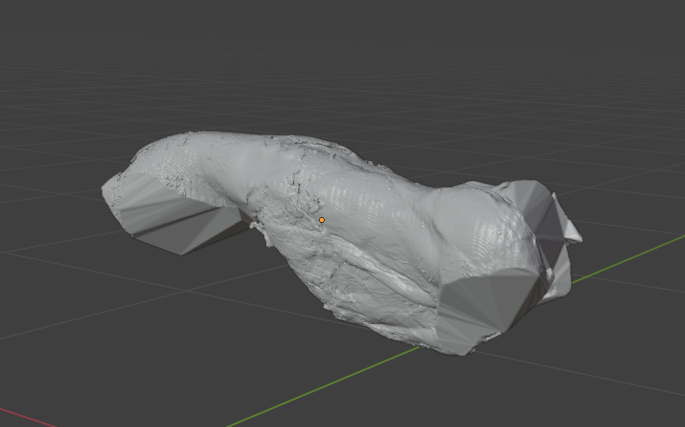
\includegraphics[width=\textwidth]{figures/cheetah_hull.png} % Add image
    \caption{The "Torso.obj" mesh from \cite{coathamConvexHullEstimation2021}, providing a 3D model of the torso of a cheetah, segmented from a CT-scan.}
    \label{fig:cheetahhull}
\end{figure}

Using the "Compute Geometric Measures" filter, Meshlab gives: \(V\) = 0.027241 \si{m^3}, center of mass = \((0.461789, -0.002036, 0.555943)\) \si{m}, and the volumetric inertia tensor as (0.000177, 0.002123, 0.002045, 0.000060, 0.000113, 0.000011) \si{m^5}. MuSkeMo gives the following outputs (setting density at 1000 \si{kg m^{-3}}): \(m\) = 27.2405 \si{kg}, center of mass = \((0.461789, -0.002036, 0.555943)\) \si{m}, and the mass inertial tensor as (0.176614, 2.12329, 2.0455, 0.060367, 0.113492, 0.010864).

The numerical values are the same, save for a factor of 1000 representing the density.

\subsection{Composite bodies and meshes}

\label{sec:compositebodyvalidation}

MuSkeMo can combine the inertial properties of several source objects into a single composite body using the (3D) parallel axes theorem \cite{valleryAdvancedDynamics2019,ruinaMechanicsToolsetStatics2019}. Here, we will compute the values manually for the situation pictured in Fig. \ref{fig:icoandsphere}, and compare the computations by MuSkeMo.


\begin{figure}[htbp]
    \centering
    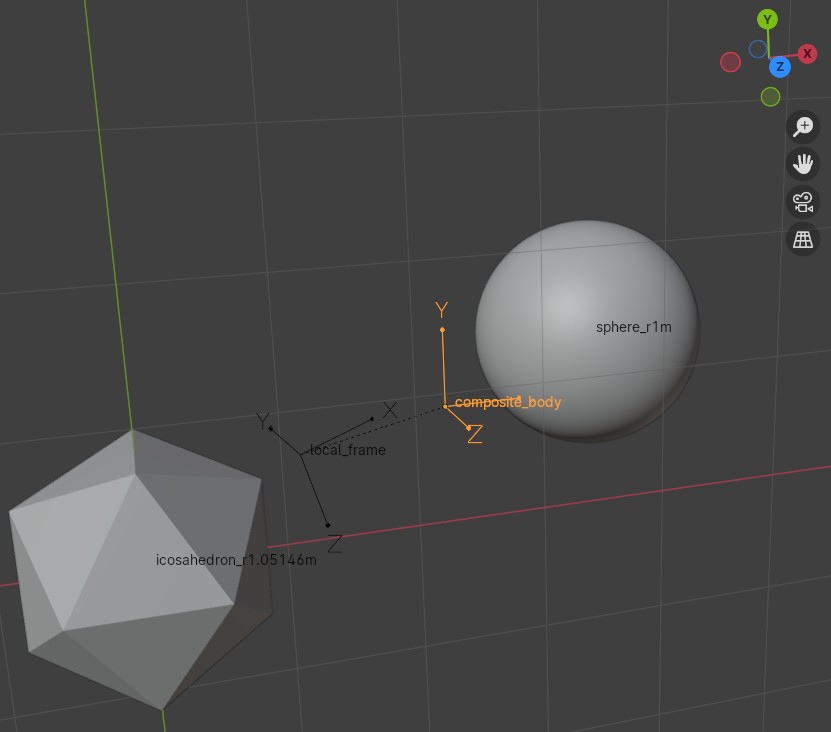
\includegraphics[width=\textwidth]{figures/composite_body.png} % Add image
    \caption{The icosahedron, sphere, composite body, and local frame described in sections \ref{sec:inpropvalidation}, \ref{sec:compositebodyvalidation}, and \ref{sec:framevalidation}}
    \label{fig:icoandsphere}
\end{figure}


Consider the icosahedron and sphere from \ref{sec:inpropvalidation}. The icosahedron has mass \(m_{i}\) = 2536.13 \si{kg}, center of mass \(\vec{c_{i}} =  (0,0,0)\)  \si{m}, and its inertia tensor:

\begin{equation}
    \mathbf{I}_{i/c,{\mathcal{G}}} = \mqty(
    734.063 & 0 & 0 \\
    0 & 734.063 & 0 \\
    0 & 0 & 734.063
    ).
\end{equation}

For the inertia tensor, the subscript \(i\) denotes the icosahedron, and \(c\) signifies the inertia is given with respect to its center of mass. Like in \ref{sec:eulerangles}, \(\mathcal{G}\) signifies the tensor is expressed in the global frame.

The sphere has mass \(m_{s}\) = 4188.79 \si{kg}, center of mass \(\vec{c_{s}} =\) (4,1,-1.5) \si{m}, and its inertia tensor:

\begin{equation}
    \mathbf{I}_{s/c,{\mathcal{G}}} = \mqty(
    1675.52 & 0 & 0 \\
    0 & 1675.52 & 0 \\
    0 & 0 & 1675.52
    )
\end{equation}

The combined center of mass \(\vec{c_{c}}\) is:

\begin{equation}
    \frac{m_{i} \cdot \vec{c_{i}} + m_{s} \cdot \vec{c_{s}}}{m_{i} + m_{s}} = \vec{c_{c}},
\end{equation}

which is at (2.4915, 0.6229, -0.9343) \si{m} in the \(\mathcal{G}\)-frame when we compute it manually. In MuSkeMo, the inertial properties computed for the icosahedron and the sphere in \ref{sec:inpropvalidation} can be assigned to a single body in the Body panel (see \ref{sec:bodypanel}). When their rigid body parameters are assigned to a BODY named "composite\_body", the combined center of mass is computed as (2.4915, 0.6229,-0.9343) \si{m}. 

The combined inertial parameters can be calculated manually using the 3D parallel axes theorem \cite{valleryAdvancedDynamics2019,ruinaMechanicsToolsetStatics2019}. To fully write out the equation, it is useful to first define:

\begin{equation}
\vec{d_{i//c}} = \vec{c_i} - \vec{c_c},
\end{equation}

and a matrix constructed of its elements:

\begin{equation}
    \mathbf{D}_{i//c,\mathcal{G}} = \mqty(
        \vec{d_{i//c, y}}^2 + \vec{d_{i//c, z}}^2& - \vec{d_{i//c, x}} \cdot \vec{d_{i//c, y}} & - \vec{d_{i//c, x}} \cdot \vec{d_{i//c, z}} \\
        - \vec{d_{i//c, x}} \cdot \vec{d_{i//c, y}} &\vec{d_{i//c, x}}^2 + \vec{d_{i//c, z}}^2& - \vec{d_{i//c, y}} \cdot \vec{d_{i//c, z}}  \\
        - \vec{d_{i//c, x}} \cdot \vec{d_{i//c, z}}  & - \vec{d_{i//c, y}} \cdot \vec{d_{i//c, z}}  & \vec{d_{i//c, x}}^2 + \vec{d_{i//c, y}}^2
    ).
\end{equation}

The matrix \(\mathbf{D}_{s//c,\mathcal{G}}\) is similarly constructed from \(\vec{{d_{s//c}}}\). It is also possible to define \(\vec{d_{c//i}}\) and its respective matrix \(\mathbf{D}_{c//i,\mathcal{G}}\), but because each term is either squared or multiplied with another term, this gives the same result.

To calculate \(\mathbf{I}_{c/c,{\mathcal{G}}}\), the combined inertial properties with respect to \(\vec{c_c}\) in the \(\mathcal{G}\)-frame, we apply the following:

\begin{equation}
\mathbf{I}_{c/c,{\mathcal{G}}} = \mathbf{I}_{i/c,{\mathcal{G}}} + m_i \cdot \mathbf{D}_{i//c,\mathcal{G}} +  \mathbf{I}_{s/c,{\mathcal{G}}} + m_s \cdot \mathbf{D}_{s//c,\mathcal{G}},
\end{equation}
which is the 3D parallel axes theorem \cite{valleryAdvancedDynamics2019,ruinaMechanicsToolsetStatics2019}.

Manually calculated, the inertial properties are:
(7543.59, 31239.0, 29264.4, -6318.78, 9478.17, 2369.54) \si{kg m^2}, using the same element order as defined in \ref{sec:body}. After applying the parallel axes theorem, MuSkeMo computes the inertial properties as: (7543.47,31238.7,29264.1,-6318.73,9478.10,2369.53) \si{kg m^2}.

As an extra internal validation step, it is also possible to combine the meshes from Fig. \ref{fig:icoandsphere} into a single composite mesh, using Blender's join command. If inertial properties for this composite mesh are computed using MuSkeMo, MuSkeMo treats them as a single (but disjointed) mesh, and uses Eberly's algorithm to compute the combined rigid body parameters. This gives numerically identical results, even though the "composite body" approach uses the parallel axes theorem to combine two mesh inertial properties, whereas the "composite mesh" approach computes the inertial properties as if they were one single mesh.

\subsection{Re-expressing matrices and vectors in arbitary frames}
\label{sec:framevalidation}
When assigning a local frame (see \ref{sec:frame}) to a BODY , MuSkeMo also expresses the parameters of all associated model components with respect to that local frame (see \ref{sec:DataTypes}). The scripts that compute these matrices are reused throughout MuSkeMo, so we will demonstrate their implementation by expressing the composite rigid body parameters from \ref{sec:compositebodyvalidation} with respect to a local frame.

The frame is pictured in \ref{fig:icoandsphere}. The frame's global position is \(\vec{r_f}\) = (1,1,1) \si{m}. Its Euler angles are 45 \si{\degree} (\( \phi_x \)), 10 \si{\degree} (\( \phi_y \)), and 25 \si{\degree} (\( \phi_z \)), see \ref{sec:eulerangles} for a full treatment on Euler angles in MuSkeMo. Thus, the rotation matrix \({}^{\mathcal{G}} \mathbf{R}_{\mathcal{B}}\), which rotates a vector from the local frame to the global frame, follows from equation \ref{eq:grbmatrix} as:


\begin{equation}
    {}^{\mathcal{G}} \mathbf{R}_{\mathcal{B}} =
    \mqty(
    0.892539 & -0.416198 & 0.173648 \\
    0.410120 & 0.588964 & -0.696364 \\
    0.187553 & 0.692749 & 0.696364
    )
\end{equation}

To express the combined center of mass \(\vec{c_{c}}\) from \ref{sec:compositebodyvalidation} with respect to the local frame, we will start by explicitly defining in which frames the vectors are expressed, \(\mathcal{G}\) for the global frame, and \(\mathcal{B}\) for the local frame (the B stands for body-fixed). To compute the transformation manually, we use:

\begin{equation}
\vec{c}_{c,\mathcal{B}} = {}^{\mathcal{B}} \mathbf{R}_{\mathcal{G}} \cdot (\vec{c}_{c,\mathcal{G}} - \vec{r}_{f,\mathcal{G}}).
\end{equation}

Calculated manually, this gives: (0.813771, -2.18287, -0.825374) \si{m}. When assigning the local frame to the composite body, MuSkeMo computes: (0.813736, -2.18285, -0.825365) \si{m}. 

To re-express \(\mathbf{I}_{c/c,{\mathcal{G}}}\) in the \(mathcal{B}\)-frame (but still with respect to the combined center of mass), we apply equation \ref{eq:similaritytransformation} (as can be found in standard mechanics textbooks \cite{valleryAdvancedDynamics2019}):

\begin{equation}
    \mathbf{I}_{c/c,{\mathcal{B}}} = {}^{\mathcal{B}} \mathbf{R}_{\mathcal{G}} \cdot \mathbf{I}_{c/c,{\mathcal{G}}} \cdot {}^{\mathcal{G}} \mathbf{R}_{\mathcal{B}}.
\end{equation}

Manual calculations give: (11205.0, 25752.7, 31089.3, 12358.1, 6113.85, -3495.72) \si{kg m^2}. MuSkeMo computes: (11204.8, 25752.4, 31089.0, 12358.0, 6113.81, -3495.70) \si{kg m^2}.


\subsection{Muscle moment arms}
\label{sec:momentarmvalidation}

Several definitions of muscle moment arms exist \cite{anDeterminationMuscleOrientations1984}. MuSkeMo computes the moment arms using the principle of virtual work \cite{anDeterminationMuscleOrientations1984,storaceFunctionalAnalysisRole1979}. For muscle \(m\) crossing a joint with joint angle \(\phi_j\), the moment arm \(r_m\) is determined by changes in the muscle's length \(l_m\) as a function of the the joint angle:

\begin{equation}
r_m = -dl_m / d\phi_j
\end{equation}
\label{eq:momentarm}

The minus sign in eq. \ref{eq:momentarm} appears due to the convention in musculoskeletal simulators to define muscle contractile force as a positive scalar, even though muscle contraction results in a negative change in length.

Accurate computations of moment arms therefore require correct application of local frames, positions and orientations, require accurate changes in muscle point positions when the joints are rotated, and also require accurate computations of the instantaneous muscle lengths in all of the different joint poses. Fig. \ref{fig:momentarmsindividual} compares the moment arms computed by MuSkeMo after importing an OpenSim model, to the moment arms of the same model computed by OpenSim 4.0 using the Matlab api. These are the same data that are combined into three plots in Fig. \ref{fig:momentarmscombined}. Note that the moment arms computed by MuSkeMo will only match those computed by OpenSim if the model only uses wrapping cylinders, with each wrapped section separated by a curve point (or if the model uses no wrapping at all).

\begin{figure}[htbp]
    %\vspace{-155pt}
    \centering
    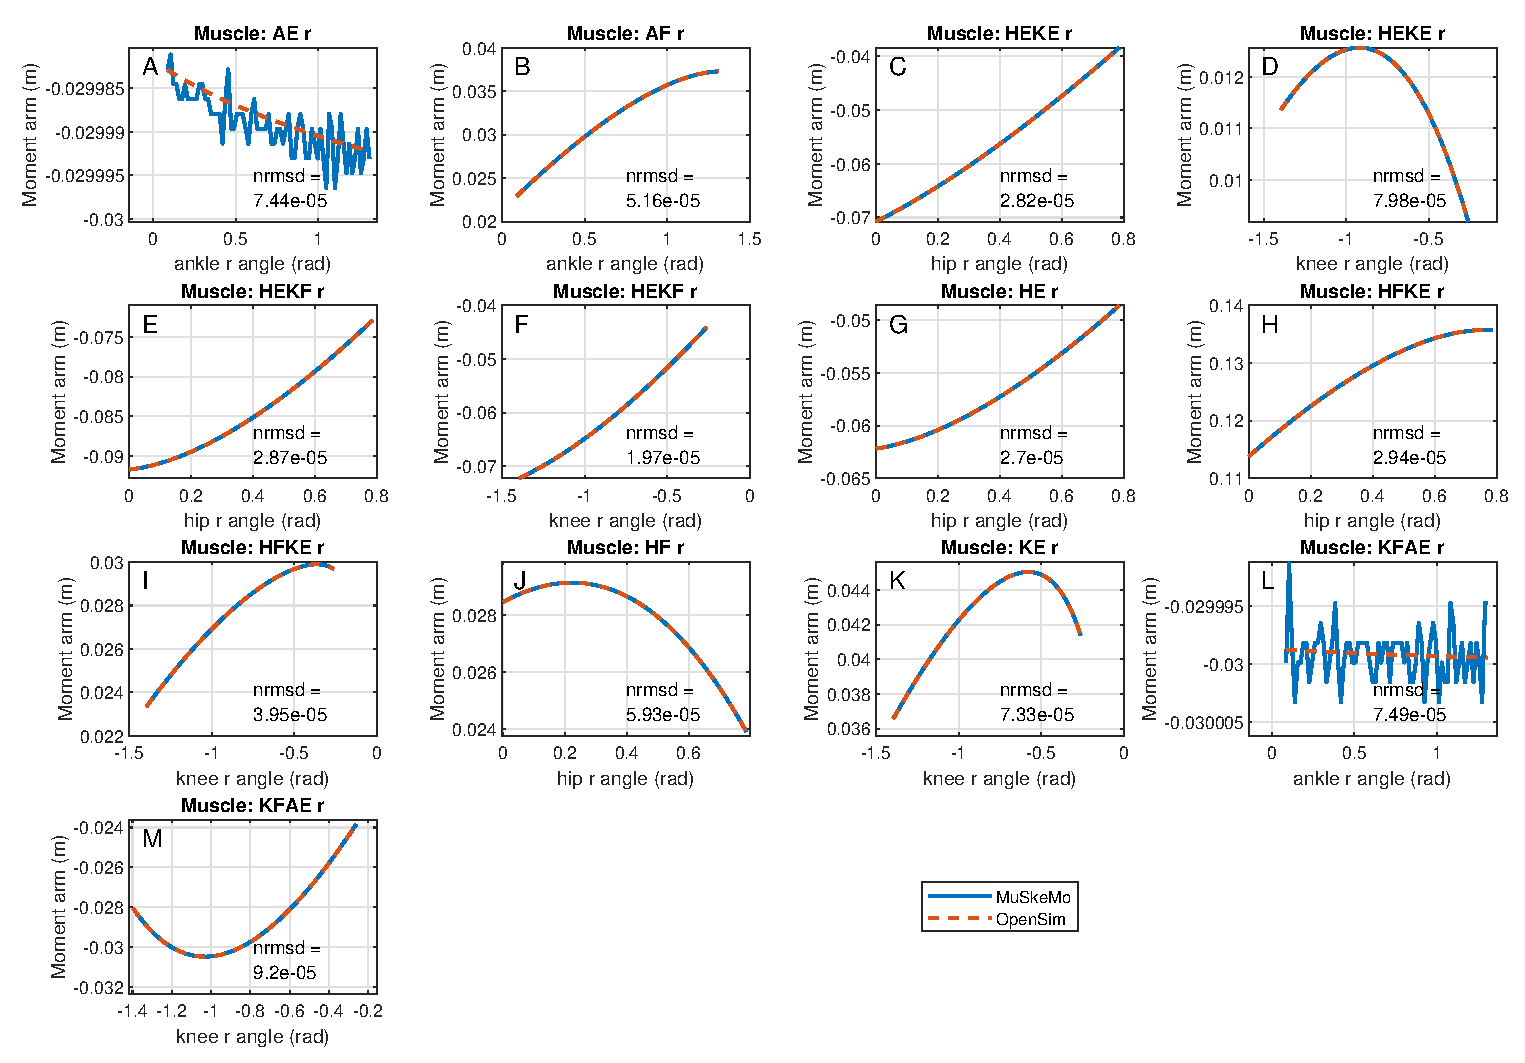
\includegraphics[width=1\textwidth]{figures/emu_momentarms_individual_v2.eps} % Add image
    \caption{Individual muscle moment arms of the emu model from \cite{vanbijlertMusclecontrolledPhysicsSimulations2024}, computed by MuSkeMo and exported as .csv files, compared to those computed by OpenSim 4.0 using the Matlab API. nrmsd stands for "normalized root mean squared differences", rmsd is normalized by the mean value of the moment arm. The average nmrsd over all muscles was 0.0052\% of the moment arm magnitudes.
    Panels A and L show that the moment arms are slightly noisy (in the order of 0.015\% the magnitude of the moment arm) when wrapping determines the moment arms in question. As evidenced by similar values of nrmsd, this noise is too small to be relevant in most practical applications (e.g., compare this figure to the same data plotted in Fig. \ref{fig:momentarmscombined}, where the noise is not perceptible over a larger range).   
    The python script that performs this moment arm analysis is provided in the Utilities folder \ref{sec:muskemoutilities}}.
    \label{fig:momentarmsindividual}
\end{figure}

The OpenSim model used for this comparison was the emu model from \cite{vanbijlertMusclecontrolledPhysicsSimulations2024}, specifically \texttt{Dromaius\_model\_ \allowbreak v4\_intermed.\allowbreak osim}. Fig. \ref{fig:momentarmsindividual} shows that all the moment arms are numerically identical within expected precision for Blender, as evidenced by the normalized root mean square differences (nrmsd) not exceeding \(9.2 \cdot 10^{-4}\), or 0.0092\% of the moment arm magnitudes, with an average of 0.0052\% over all the muscles. To compute nrmsd, rmsd was normalized by the mean of the moment arm of each muscle.

Fig. \ref{fig:momentarmsindividual} also shows that the moment arms in panels A and L are somewhat noisy. Closer inspection of the vertical axes of those panels reveals that the moment arms are nearly constant for those muscles (\~ -0.03 \si{m}), because the moment arms are determined by a cylinder with constant diameter radius (0.03 \si{m}). Thus, the noise is numerically insignificant (in the order of ~0.015\% of the moment arm magnitude). The noise is so small in magnitude that it is not visible when plotting multiple muscles in the same plot, with more informative ranges on the y axis (Fig. \ref{fig:momentarmscombined}).

While the noise is small enough to make no difference in a practical sense, it is explicitly pointed out here, because readers who want to use MuSkeMo's moment arms directly for their own simulations may want to smooth the moment arms first. The noisy moment arms for wrapping muscles are likely caused by wrapping node (see sec. \ref{sec:musclewrapping}). A likely possibility is that the many mathematical operations that are performed in the node on single precision digits introduce floating point errors (see \nameref{sec:precision}). Another possible culprit may be inaccuracy of the Raycasting operation that geometrically determines intersections between a wrapping geometry and a muscle curve.

The python script (to be run in Blender's script editor) that generates the muscle analysis is provided in MuSkeMo's utilities folder as an example script that calls MuSkeMo's API (sec. \ref{sec:muskemoutilities}). The Matlab script that generates the plots from Figs. \ref{fig:momentarmscombined} and \ref{fig:momentarmsindividual} is also provided.

\newpage
\section{Acknowledgements}

\section*{References}
\addcontentsline{toc}{section}{References} % Add to TOC
\printbibliography[heading=none] % Suppress the default heading


\end{document}
